\chapter{树}

\section{树}

\subsection{树(Tree)}

许多逻辑关系并不是简单的线性关系,在实际场景中,常常存在着一对多,甚至多对多的情况。树和图就是典型的非线性数据结构。\\

\begin{figure}[H]
	\centering
	\begin{tikzpicture}[
			level distance=2.5cm,
			level 1/.style={sibling distance=6cm},
			level 2/.style={sibling distance=2cm},
			level 3/.style={sibling distance=2cm}
		]
		\node {技术总监}
		child {
				node {项目经理A}
				child {node {员工A}}
				child {node {员工B}}
				child {node {员工C}}
			}
		child {
				node {项目经理B}
				child {node {员工D}}
				child {node {员工E}}
			};
	\end{tikzpicture}
	\caption{职级关系}
\end{figure}

这些结构都像自然界中的树一样,从同一个根衍生出许多枝干,再从每一个枝干衍生出许多更小的枝干,最后衍生出更多的叶子。\\

树是由$ n\ (n \ge 0) $个有限节点组成的一个具有层次关系的集合,当$ n = 0 $时称为空树。\\

在任意一个非空树中,有以下特点:

\begin{itemize}
	\item 有且有且仅有一个特定的结点称为根(root)。

	\item 当$ n > 1 $时,其余结点可分为$ m\ (m > 0) $个互不相交的有限集$ T_1, T_2, \dots, T_m $,其中每一个集合本身又是一棵树,并且称为根的子树(subtree)。
\end{itemize}

\vspace{0.5cm}

\subsection{树的术语}

\begin{figure}[H]
	\centering
	\begin{tikzpicture}[
			level distance=2cm,
			level 1/.style={sibling distance=4cm},
			level 2/.style={sibling distance=1.5cm},
			level 3/.style={sibling distance=1.5cm}
		]
		\node[circle,draw] {A}
		child {
				node[circle,draw] {B}
				child {
						node[circle,draw] {D}
						child {node[circle,draw] {G}}
						child {node[circle,draw] {H}}
						child {node[circle,draw] {I}}
					}
				child[missing] {}
			}
		child {
				node[circle,draw] {C}
				child {
						node[circle,draw] {E}
						child[missing] {}
						child {node[circle,draw] {J}}
					}
				child {node[circle,draw] {F}}
			};
	\end{tikzpicture}
	\caption{树}
\end{figure}

\begin{itemize}
	\item 根:没有父结点(parent)的结点。

	\item 内部结点(internal node):至少有一个子结点(child)的结点。

	\item 外部结点(external node) / 叶子结点(leaf node):没有子结点的结点。

	\item 度(degree):结点分支的个数。

	\item 路径(path):从根结点到树中某结点经过的分支构成了路径。

	\item 祖先结点(ancestors):包含父结点、父结点的父结点等。

	\item 子孙结点(descendants):包含子结点、子结点的子结点等。

	\item 深度(depth) / 高度(height):最大层级数。
\end{itemize}

\newpage

\section{二叉树}

\subsection{二叉树(Binary Tree)}

二叉树是树的一种特殊形式。二叉树的每个结点最多有两个孩子结点,即最多有2个,也可能只有1个,或者没有孩子结点。\\

二叉树结点的两个孩子结点,分别被称为左孩子(left child)和右孩子(right child)。这两个孩子结点的顺序是固定的,不能颠倒或混淆。\\

\begin{figure}[H]
	\centering
	\begin{tikzpicture}[
			level distance=1.5cm,
			level 1/.style={sibling distance=2cm},
			level 2/.style={sibling distance=1.5cm},
			level 3/.style={sibling distance=1.5cm}
		]
		\node[circle,draw] {1}
		child {
				node[circle,draw] {2}
				child {
						node[circle,draw] {4}
						child {node[circle,draw] {7}}
						child {node[circle,draw] {8}}
					}
				child {node[circle,draw] {5}}
			}
		child {
				node[circle,draw] {3}
				child[missing] {}
				child {node[circle,draw] {6}}
			};
	\end{tikzpicture}
	\caption{二叉树}
\end{figure}

二叉树还有几种特殊的形式:

\subsubsection{左斜树(left skew tree) / 右斜树(right skew tree)}

只有左子树或只有右子树的二叉树。\\

\begin{figure}[H]
	\centering
	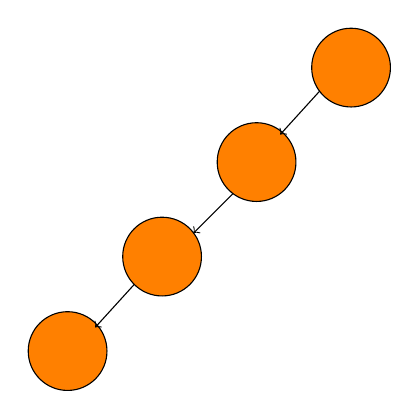
\begin{tikzpicture}
		\draw[fill=orange] (0,0) circle (0.5);
		\draw[fill=orange] (-1.2,-1.2) circle (0.5);
		\draw[fill=orange] (-2.4,-2.4) circle (0.5);
		\draw[fill=orange] (-3.6,-3.6) circle (0.5);

		\draw[->] (-0.4,-0.3) -- (-0.9,-0.85);
		\draw[->] (-1.5,-1.6) -- (-2,-2.1);
		\draw[->] (-2.75,-2.75) -- (-3.25,-3.3);
	\end{tikzpicture}
	\caption{左斜树}
\end{figure}

\subsubsection{满二叉树(full binary tree)}

所有非叶子结点都存在左右孩子,并且所有叶子结点都在同一层。\\

\begin{figure}[H]
	\centering
	\begin{tikzpicture}[
			level distance=1.5cm,
			level 1/.style={sibling distance=4cm},
			level 2/.style={sibling distance=2cm},
			level 3/.style={sibling distance=1cm}
		]
		\node[circle,draw] {1}
		child {
				node[circle,draw] {2}
				child {
						node[circle,draw] {4}
						child {node[circle,draw] {8}}
						child {node[circle,draw] {9}}
					}
				child {
						node[circle,draw] {5}
						child {node[circle,draw] {10}}
						child {node[circle,draw] {11}}
					}
			}
		child {
				node[circle,draw] {3}
				child {
						node[circle,draw] {6}
						child {node[circle,draw] {12}}
						child {node[circle,draw] {13}}
					}
				child {
						node[circle,draw] {7}
						child {node[circle,draw] {14}}
						child {node[circle,draw] {15}}
					}
			};
	\end{tikzpicture}
	\caption{满二叉树}
\end{figure}

\subsubsection{完全二叉树}

对于一个有n个结点的二叉树,按层级顺序编号,则所有结点的编号从1到n,完全二叉树所有结点和同样深度的满二叉树的编号从1到n的结点位置相同。简单来说,就是除最后一层外,其它各层的结点数都达到最大,并且最后一层从右向左连续缺少若干个结点。\\

\begin{figure}[H]
	\centering
	\begin{tikzpicture}[
			level distance=1.5cm,
			level 1/.style={sibling distance=4cm},
			level 2/.style={sibling distance=2cm},
			level 3/.style={sibling distance=1cm}
		]
		\node[circle,draw] {1}
		child {
				node[circle,draw] {2}
				child {
						node[circle,draw] {4}
						child {node[circle,draw] {8}}
						child {node[circle,draw] {9}}
					}
				child {
						node[circle,draw] {5}
						child {node[circle,draw] {10}}
						child {node[circle,draw] {11}}
					}
			}
		child {
				node[circle,draw] {3}
				child {
						node[circle,draw] {6}
						child {node[circle,draw] {12}}
						child[missing] {}
					}
				child {node[circle,draw] {7}}
			};
	\end{tikzpicture}
	\caption{完全二叉树}
\end{figure}

\vspace{0.5cm}

\subsection{二叉树的存储结构}

二叉树既可以通过链式存储,也可以使用数组存储:

\subsubsection{链式存储结构}

一个结点最多可以指向左右两个孩子结点,所以二叉树的每一个结点包含三个部分:

\begin{itemize}
	\item 存储数据的数据域data
	\item 指向左孩子的指针left
	\item 指向右孩子的指针right
\end{itemize}

\begin{figure}[H]
	\centering
	\begin{tikzpicture}
		\draw (0,0) rectangle (3,2);
		\draw (-1,-4) rectangle (-4,-2);
		\draw (4,-4) rectangle (7,-2);

		\draw (0,1) -- (3,1);
		\draw(1.5,1) -- (1.5,0);
		\draw (-4,-3) -- (-1,-3);
		\draw(-2.5,-4) -- (-2.5,-3);
		\draw (7,-3) -- (4,-3);
		\draw(5.5,-4) -- (5.5,-3);

		\draw (1.5,1.5) node{data};
		\draw (0.75,0.5) node{left};
		\draw (2.25,0.5) node{right};
		\draw (-2.5,-2.5) node{data};
		\draw (-3.25,-3.5) node{left};
		\draw (-1.75,-3.5) node{right};
		\draw (5.5,-2.5) node{data};
		\draw (4.75,-3.5) node{left};
		\draw (6.25,-3.5) node{right};

		\draw[->] (0.5,0.2) -- (-2,-2.5);
		\draw[->] (2.5,0.2) -- (5,-2.5);
	\end{tikzpicture}
	\caption{链式存储结构}
\end{figure}

\subsubsection{数组存储}

按照层级顺序把二叉树的结点放到数组中对应的位置上。如果某一结点的左孩子或右孩子空缺,则数组的相应位置也空出来。\\

\begin{figure}[H]
	\centering
	\begin{tikzpicture}[
			level distance=1.5cm,
			level 1/.style={sibling distance=4cm},
			level 2/.style={sibling distance=2cm},
			level 3/.style={sibling distance=1cm}
		]
		\node[circle,draw] {1}
		child {
				node[circle,draw] {2}
				child {
						node[circle,draw] {4}
						child[missing] {}
						child {node[circle,draw] {8}}
					}
				child {node[circle,draw] {5}}
			}
		child {
				node[circle,draw] {3}
				child[missing] {}
				child {node[circle,draw] {6}}
			};
	\end{tikzpicture}
\end{figure}

\begin{figure}[H]
	\centering
	\begin{tikzpicture}[]
		\draw[-] (0,0) rectangle (9,1);
		\draw[-] (1,0) -- (1,1);
		\draw[-] (2,0) -- (2,1);
		\draw[-] (3,0) -- (3,1);
		\draw[-] (4,0) -- (4,1);
		\draw[-] (5,0) -- (5,1);
		\draw[-] (6,0) -- (6,1);
		\draw[-] (7,0) -- (7,1);
		\draw[-] (8,0) -- (8,1);

		\draw (0.5,0.5) node{1};
		\draw (1.5,0.5) node{2};
		\draw (2.5,0.5) node{3};
		\draw (3.5,0.5) node{4};
		\draw (4.5,0.5) node{5};
		\draw (6.5,0.5) node{6};
		\draw (8.5,0.5) node{8};

		\draw (0.5,-0.5) node{0};
		\draw (1.5,-0.5) node{1};
		\draw (2.5,-0.5) node{2};
		\draw (3.5,-0.5) node{3};
		\draw (4.5,-0.5) node{4};
		\draw (5.5,-0.5) node{5};
		\draw (6.5,-0.5) node{6};
		\draw (7.5,-0.5) node{7};
		\draw (8.5,-0.5) node{8};
	\end{tikzpicture}
	\caption{数组存储}
\end{figure}

采用数组存储可以更方便地定位二叉树的孩子结点和父结点。假设一个父结点的下标是parent,那么它的左孩子结点的下标就是2 * parent + 1,右孩子结点的下标就是2 * parent + 2。反过来,假设一个左孩子结点的下标是leftChild,那么它的父结点的下标就是(leftChild - 1) / 2。\\

但是,对于一个稀疏的二叉树来说,用数组表示法是非常浪费空间的。对于一种特殊的完全二叉树——二叉堆而言,就是使用数组进行存储的。

\newpage

\section{二叉树的遍历}

\subsection{二叉树的遍历}

在计算机程序中,遍历(traversal)本身是一个线性操作,所以遍历同样具有线性结构的数组或链表是一件轻而易举的事情。\\

反观二叉树,是典型的非线性数据结构,遍历时需要把非线性关联的结点转化成一个线性的序列,以不同的方式来遍历,遍历出的序列顺序也不同。\\

二叉树的遍历方式分为4种:

\begin{enumerate}
	\item 前序遍历(pre-order):访问根结点,遍历左子树,遍历右子树。

	\item 中序遍历(in-order):遍历左子树,访问根结点,遍历右子树。

	\item 后序遍历(post-order):遍历左子树,遍历右子树,访问根结点。

	\item 层次遍历(level-order):按照从根结点到叶子结点的层次关系,一层一层横向遍历。
\end{enumerate}

\vspace{0.5cm}

\subsection{前序遍历}

二叉树的前序遍历,首先访问根结点然后遍历左子树,最后遍历右子树。在遍历左、右子树时,仍然先访问根结点,然后遍历左子树,最后遍历右子树,如果结点为空则返回。\\

\begin{figure}[H]
	\centering
	\begin{tikzpicture}[
			level distance=1.5cm,
			level 1/.style={sibling distance=4cm},
			level 2/.style={sibling distance=2cm},
			level 3/.style={sibling distance=1cm}
		]
		\node[circle,draw] {1}
		child {
				node[circle,draw] {2}
				child {
						node[circle,draw] {4}
					}
				child {
						node[circle,draw] {5}
					}
			}
		child {
				node[circle,draw] {3}
				child[missing] {}
				child {node[circle,draw] {6}}
			};

		\draw[color=red] (-0.7,0) node{1};
		\draw[color=red] (-2.75,-1.5) node{2};
		\draw[color=red] (-3.75,-3) node{3};
		\draw[color=red] (-1.75,-3) node{4};
		\draw[color=red] (1.25,-1.5) node{5};
		\draw[color=red] (2.25,-3) node{6};
	\end{tikzpicture}
	\caption{前序遍历}
\end{figure}

\mybox{前序遍历}

\begin{lstlisting}[language=C]
void preOrder(BST *root) {
    if(!root) {
        return;
    }
    printf("%d ", root->data);
    preOrder(root->left);
    preOrder(root->right);
}
\end{lstlisting}

\vspace{0.5cm}

\subsection{中序遍历}

二叉树的中序遍历,首先遍历左子树,然后访问根结点,最后遍历右子树,如果结点为空则返回。\\

\begin{figure}[H]
	\centering
	\begin{tikzpicture}[
			level distance=1.5cm,
			level 1/.style={sibling distance=4cm},
			level 2/.style={sibling distance=2cm},
			level 3/.style={sibling distance=1cm}
		]
		\node[circle,draw] {1}
		child {
				node[circle,draw] {2}
				child {
						node[circle,draw] {4}
					}
				child {
						node[circle,draw] {5}
					}
			}
		child {
				node[circle,draw] {3}
				child[missing] {}
				child {node[circle,draw] {6}}
			};

		\draw[color=red] (-0.7,0) node{4};
		\draw[color=red] (-2.75,-1.5) node{2};
		\draw[color=red] (-3.75,-3) node{1};
		\draw[color=red] (-1.75,-3) node{3};
		\draw[color=red] (1.25,-1.5) node{5};
		\draw[color=red] (2.25,-3) node{6};
	\end{tikzpicture}
	\caption{中序遍历}
\end{figure}

\mybox{中序遍历}

\begin{lstlisting}[language=C]
void inOrder(BST *root) {
    if(!root) {
        return;
    }
    inOrder(root->left);
    printf("%d ", root->data);
    inOrder(root->right);
}
\end{lstlisting}

\vspace{0.5cm}

\subsection{后序遍历}

二叉树的后序遍历,首先遍历左子树,然后遍历右子树,最后访问根结点,如果结点为空则返回。\\

\begin{figure}[H]
	\centering
	\begin{tikzpicture}[
			level distance=1.5cm,
			level 1/.style={sibling distance=4cm},
			level 2/.style={sibling distance=2cm},
			level 3/.style={sibling distance=1cm}
		]
		\node[circle,draw] {1}
		child {
				node[circle,draw] {2}
				child {
						node[circle,draw] {4}
					}
				child {
						node[circle,draw] {5}
					}
			}
		child {
				node[circle,draw] {3}
				child[missing] {}
				child {node[circle,draw] {6}}
			};

		\draw[color=red] (-0.7,0) node{6};
		\draw[color=red] (-2.75,-1.5) node{3};
		\draw[color=red] (-3.75,-3) node{1};
		\draw[color=red] (-1.75,-3) node{2};
		\draw[color=red] (1.25,-1.5) node{5};
		\draw[color=red] (2.25,-3) node{4};
	\end{tikzpicture}
	\caption{后序遍历}
\end{figure}

\mybox{后序遍历}

\begin{lstlisting}[language=C]
void postOrder(BST *root) {
    if(!root) {
        return;
    }
    postOrder(root->left);
    postOrder(root->right);
    printf("%d ", root->data);
}
\end{lstlisting}

\vspace{0.5cm}

\subsection{二叉树遍历非递归实现}

绝大多数可以用递归解决的问题,其实都可以用栈来解决,因为递归和栈都有回溯的特性。\\

以二叉树的中序遍历为例。当遇到一个结点时,就把它入栈,并去遍历它的左子树。当左子树遍历结束后,从栈顶弹出这个结点并访问它,然后按其右指针再去中序遍历该结点的右子树。\\

\mybox{中序遍历(非递归)}

\begin{lstlisting}[language=Java]
public void inOrderNonRecursive(BSTNode node) {
    Stack s = new Stack();
    while(node != null || !s.empty()) {
        // 一直向左并将沿途结点压入堆栈
        while(node != null) {
            s.push(node);
            node = node.left;
        }
        if(!s.empty()) {
            node = s.pop();					   //结点弹出堆栈
            System.out.println(node.data);		// 访问结点
            node = node.right;				   // 转向右子树
        }
    }
}
\end{lstlisting}

\vspace{0.5cm}

\subsection{层次遍历}

二叉树同一层次的结点之间是没有直接关联的,需要队列来辅助完成层序遍历。\\

层次遍历从根结点开始首先将根结点入队,然后开始循环执行以下操作直到队列为空:结点出队、访问该结点、其左右儿子入队。\\

\mybox{层次遍历}

\begin{lstlisting}[language=Java]
public void levelOrder(BSTNode node) {
    if(node == null) {
        return;
    }
    
    Queue q = new Queue();
    q.enqueue(node);
    while(!q.empty()) {
        node = q.dequeue();
        System.out.println(node.data);		// 访问结点
        if(node.left != null) {
            q.enqueue(node.left);
        }
        if(node.right != null) {
            q.enqueue(node.right);
        }
    }
}
\end{lstlisting}

\newpage

\section{二叉搜索树}

\subsection{二叉搜索树(Binary Search Tree)}

二叉搜索树,也称二叉查找树或二叉排序树,可以是一棵空树。\\

如果不为空树,那么二叉搜索树满足以下性质:

\begin{enumerate}
	\item 非空左子树的所有结点的值小于其根结点的值。
	\item 非空右子树的所有结点的值大于其根结点的值。
	\item 左、右子树均是二叉搜索树。
\end{enumerate}

\begin{figure}[H]
	\centering
	\begin{tikzpicture}[
			level distance=1.5cm,
			level 1/.style={sibling distance=4cm},
			level 2/.style={sibling distance=2cm},
			level 3/.style={sibling distance=1cm}
		]
		\node[circle,draw] {6}
		child {
				node[circle,draw] {3}
				child {
						node[circle,draw] {2}
						child {node[circle,draw] {1}}
						child[missing] {}
					}
				child {node[circle,draw] {4}}
			}
		child {
				node[circle,draw] {8}
				child {node[circle,draw] {7}}
				child {node[circle,draw] {9}}
			};
	\end{tikzpicture}
	\caption{二叉搜索树}
\end{figure}

\vspace{0.5cm}

\subsection{查找结点}

在二叉搜索树中查找一个元素从根结点开始,如果树为空,返回NULL。\\

如果树不为空,则将根结点的值和被查找的key值进行比较:

\begin{enumerate}
	\item 如果key值小于根结点的值,只需在左子树中继续查找。
	\item 如果key值大于根结点的值,只需在右子树中继续查找。
	\item 如果key值与根结点的值相等,查找成功。
\end{enumerate}

\mybox{查找结点(递归)}

\begin{lstlisting}[language=C]
Node* search(Node *root, dataType val) {
    if(!root) {
        return NULL;
    }
    if(val == root->data) {
        return root;
    } else if(val < root->data) {
        return search(root->left, val);
    } else {
        return search(root->right, val);
    }
}
\end{lstlisting}

由于非递归函数的执行效率高,可将尾递归(在函数最后才使用递归返回)的函数改为迭代函数。\\

\mybox{查找结点(迭代)}

\begin{lstlisting}[language=C]
Node* search(Node *root, dataType val) {
    if(!root) {
        return NULL;
    }  
    while(root) {
        if(root->data == val) {
            return root;
        } else if(val < root->data) {
            root = root->left;
        } else {
            root = root->right;
        }
    }
}
\end{lstlisting}

\vspace{0.5cm}

\subsection{查找最小值和最大值}

二叉搜索树中,最小值一定在树的最左分枝的叶子结点上,最大值一定在树的最右分枝的叶子结点上。\\

\mybox{查找最小值(递归)}

\begin{lstlisting}[language=C]
Node* findMin(Node *root) {
    if(!root) {
        return NULL;
    } else if(!root->left) {
        return root;
    } else {
        return findMin(root->left);		//沿左分枝继续查找
    }
}
\end{lstlisting}

\vspace{0.5cm}

\mybox{查找最大值(迭代)}

\begin{lstlisting}[language=C]
Node* findMax(Node *root) {
    if(!root) {
        return NULL;
    } 
    while(root->right) {
        root = root->right;
    }
    return root;
}
\end{lstlisting}

\vspace{0.5cm}

\subsection{插入结点}

在二叉搜索树中插入结点与查找的算法相似,需要找到插入的位置并将新结点插入。\\

\mybox{插入结点}

\begin{lstlisting}[language=C]
BST* insert(BST *root, dataType val) {
    // 空树,插入结点设为树根
    if(!root) {
        return init(val);
    }
    if(val < root->data) {
        root->left = insert(root->left, val);
    } else {
        root->right = insert(root->right, val);
    }
    return root;
}
\end{lstlisting}

\newpage

\section{哈夫曼树}

\subsection{哈夫曼树(Huffman Tree)}

树的每一个结点都可以拥有自己的权值(weight),假设二叉树有n个叶子结点,每个叶子结点都带有权值$ w_k $,从根结点到每个叶子结点的长度为$ l_k $,则树的带权路径长度(WPL, Weighted Path Length)为:

$$
	WPL = \sum_{k=1}^n w_k l_k
$$

哈夫曼树是由麻省理工学院的哈夫曼博士于1952年发明的,哈夫曼树是在叶子结点和权重确定的情况下,带权路径长度最小的二叉树,也被称为最优二叉树。\\

例如,有五个叶子结点,它们的权值为\{1, 2, 3, 4, 5\},用此权值序列可以构造出形状不同的多个二叉树。\\

\begin{figure}[H]
	\centering
	\begin{tikzpicture}[iv/.style={draw,fill=red!50,circle,minimum size=20pt,inner
					sep=0pt,text=black},ev/.style={draw,fill=yellow,rectangle,minimum
					size=20pt,inner sep=0pt,text=black}]
		\node[iv]{}
		child {node[iv]{}
				child {node[iv]{}
						child {node[iv]{}
								child {node[ev]{1}}
								child {node[ev]{2}}
							}
						child {node[ev]{3}}
					}
				child [missing]
				child {node[ev]{4}}
			}
		child [missing]
		child [missing]
		child {node[ev]{5}};
	\end{tikzpicture}
	\caption{WPL = 5 * 1 + 4 * 2 + 3 * 3 + 2 * 4 + 1 * 4 = 34}
\end{figure}

\begin{figure}[H]
	\centering
	\begin{tikzpicture}[iv/.style={draw,fill=red!50,circle,minimum size=20pt,inner
					sep=0pt,text=black},ev/.style={draw,fill=yellow,rectangle,minimum
					size=20pt,inner sep=0pt,text=black}]
		\node[iv]{}
		child {node[iv]{}
				child {node[iv]{}
						child {node[iv]{}
								child {node[ev]{5}}
								child {node[ev]{4}}
							}
						child {node[ev]{3}}
					}
				child [missing]
				child {node[ev]{2}}
			}
		child [missing]
		child [missing]
		child {node[ev]{1}};
	\end{tikzpicture}
	\caption{WPL = 1 * 1 + 2 * 2 + 3 * 3 + 4 * 4 + 5 * 4 = 50}
\end{figure}

\begin{figure}[H]
	\centering
	\begin{tikzpicture}[iv/.style={draw,fill=red!50,circle,minimum size=20pt,inner
					sep=0pt,text=black},ev/.style={draw,fill=yellow,rectangle,minimum
					size=20pt,inner sep=0pt,text=black}]
		\node[iv]{}
		child {node[iv]{}
				child {node[iv]{}
						child {node[ev]{1}}
						child {node[ev]{2}}
					}
				child [missing]
				child {node[ev]{3}}
			}
		child [missing]
		child [missing]
		child {node[iv]{}
				child {node[ev]{4}}
				child {node[ev]{5}}
			};
	\end{tikzpicture}
	\caption{WPL = 3 * 2 + 4 * 2 + 5 * 2 + 1 * 3 + 2 * 3 = 33}
\end{figure}

怎样才能保证构建出的二叉树带权路径长度最小呢?原则上,应该让权重小的叶子结点远离树根,权重大的叶子结点靠近树根。需要注意的是,同样叶子结点所构成的哈夫曼树可能不止一棵。\\

\subsection{哈夫曼树的构造}

哈夫曼树的构造方法就是每次把权值最小的两棵二叉树合并。\\

例如有6个叶子结点,权重依次是2、3、7、9、18、25。\\

第一步:把每一个叶子结点都当成一棵独立的树(只有根结点的树),这样就形成了一个森林。

\begin{figure}[H]
	\centering
	\begin{tikzpicture}
		\draw (0,0) circle (0.5) node{2};
		\draw (2,0) circle (0.5) node{3};
		\draw (4,0) circle (0.5) node{7};
		\draw (6,0) circle (0.5) node{9};
		\draw (8,0) circle (0.5) node{18};
		\draw (10,0) circle (0.5) node{25};
	\end{tikzpicture}
\end{figure}

第二步:从森林中移除权值最小的两个结点,生成父结点,父结点的权值是这两个结点权值之和,把父结点加入森林。重复该步骤,直到森林中只有一棵树为止。\\

\begin{figure}[H]
	\centering
	\begin{tikzpicture}[
			level distance=1.5cm,
			level 1/.style={sibling distance=2cm},
			level 2/.style={sibling distance=1.5cm},
			level 3/.style={sibling distance=1.5cm}
		]
		\node[circle,draw] {5}
		child {node[circle,draw] {2}}
		child {node[circle,draw] {3}};
	\end{tikzpicture}
	\caption{合并2和3}
\end{figure}

\begin{figure}[H]
	\centering
	\begin{tikzpicture}[
			level distance=1.5cm,
			level 1/.style={sibling distance=2cm},
			level 2/.style={sibling distance=1.5cm},
			level 3/.style={sibling distance=1.5cm}
		]
		\node[circle,draw] {12}
		child {
				node[circle,draw] {5}
				child {node[circle,draw] {2}}
				child {node[circle,draw] {3}}
			}
		child {node[circle,draw] {7}};
	\end{tikzpicture}
	\caption{合并5和7}
\end{figure}

\begin{figure}[H]
	\centering
	\begin{tikzpicture}[
			level distance=1.5cm,
			level 1/.style={sibling distance=2cm},
			level 2/.style={sibling distance=1.5cm},
			level 3/.style={sibling distance=1.5cm}
		]
		\node[circle,draw] {21}
		child {node[circle,draw] {9}}
		child {
				node[circle,draw] {12}
				child {
						node[circle,draw] {5}
						child {node[circle,draw] {2}}
						child {node[circle,draw] {3}}
					}
				child {node[circle,draw] {7}}
			};
	\end{tikzpicture}
	\caption{合并9和12}
\end{figure}

\begin{figure}[H]
	\centering
	\begin{tikzpicture}[
			level distance=1.5cm,
			level 1/.style={sibling distance=2cm},
			level 2/.style={sibling distance=1.5cm},
			level 3/.style={sibling distance=1.5cm}
		]
		\node[circle,draw] {39}
		child {node[circle,draw] {18}}
		child {
				node[circle,draw] {21}
				child {node[circle,draw] {9}}
				child {
						node[circle,draw] {12}
						child {
								node[circle,draw] {5}
								child {node[circle,draw] {2}}
								child {node[circle,draw] {3}}
							}
						child {node[circle,draw] {7}}
					}
			};
	\end{tikzpicture}
	\caption{合并18和21}
\end{figure}

\begin{figure}[H]
	\centering
	\begin{tikzpicture}[
			level distance=1.5cm,
			level 1/.style={sibling distance=2cm},
			level 2/.style={sibling distance=1.5cm},
			level 3/.style={sibling distance=1.5cm}
		]
		\node[circle,draw] {64}
		child {node[circle,draw] {25}}
		child {
				node[circle,draw] {39}
				child {node[circle,draw] {18}}
				child {
						node[circle,draw] {21}
						child {node[circle,draw] {9}}
						child {
								node[circle,draw] {12}
								child {
										node[circle,draw] {5}
										child {node[circle,draw] {2}}
										child {node[circle,draw] {3}}
									}
								child {node[circle,draw] {7}}
							}
					}
			};
	\end{tikzpicture}
	\caption{合并25和39}
\end{figure}

哈夫曼树有以下几个特点:

\begin{enumerate}
	\item 没有度为1的结点。
	\item 哈夫曼树的任意非叶结点的左右子树交换后仍是哈夫曼树。
	\item 对同一组权值,可能存在不同构的两棵哈夫曼树。
\end{enumerate}

\begin{figure}[H]
	\centering
	\begin{tikzpicture}[iv/.style={draw,fill=red!50,circle,minimum size=20pt,inner
					sep=0pt,text=black},ev/.style={draw,fill=yellow,rectangle,minimum
					size=20pt,inner sep=0pt,text=black}]
		\node[iv]{}
		child {node[iv]{}
				child {node[iv]{}
						child {node[ev]{1} }
						child {node[ev]{2}}
					}
				child [missing]
				child {node[ev]{3}}
			}
		child [missing]
		child [missing]
		child {node[ev]{3}};
	\end{tikzpicture}
	\caption{WPL = 3 * 1 + 3 * 2 + 1 * 3 + 2 * 3 = 18}
\end{figure}

\begin{figure}[H]
	\centering
	\begin{tikzpicture}[iv/.style={draw,fill=red!50,circle,minimum size=20pt,inner
					sep=0pt,text=black},ev/.style={draw,fill=yellow,rectangle,minimum
					size=20pt,inner sep=0pt,text=black}]
		\node[iv]{}
		child {node[iv]{}
				child {node[ev]{1}}
				child {node[ev]{2}}
			}
		child [missing]
		child {
				node[iv]{}
				child {node[ev]{3}}
				child {node[ev]{3}}
			};
	\end{tikzpicture}
	\caption{WPL = 1 * 2 + 2 * 2 + 3 * 2 + 3 * 2 = 18}
\end{figure}

\newpage

\section{哈夫曼编码}

\subsection{哈夫曼编码(Huffman Code)}

哈夫曼编码是一种高效的编码方式,在信息存储和传输过程中用于对信息进行压缩。要理解哈夫曼编码,需要从信息存储的底层逻辑讲起。\\

计算机不是人,它不认识中文和英文,更不认识图片和视频,它唯一认识的就是0(低电平)和1(高电平)。因此,计算机上一切文字、图象、音频、视频,底层都是用二进制来存储和传输的。\\

将信息转换成计算机能够识别的二进制形式的过程被称为编码。在ASCII码中,每一个字符表示成特定的8位二进制数。例如字符串APPLE表示成8位二进制编码为01000001 01010000 01010000 01001100 01000101。\\

显然,ASCII码是一种等长编码,也就是任何字符的编码长度都相等。等长编码的有点明显,因为每个字符对应的二进制编码长度相等,所以很容易设计,也很方便读写。但是计算机的存储空间以及网络传输的带宽是有限的,等长编码最大的缺点就是编码结果太长,会占用过多资源。\\

使用不等长编码,让出现频率高的字符用的编码短一些,出现频率低的字符编码长一些,可以使编码的总长度减小。但是不等长编码是不能随意设计的,如果一个字符的编码恰好是另一个字符编码的前缀,就会产生歧义的问题。\\

哈夫曼编码就是一种不等长的编码,并且任何一个字符的编码都不是另一个字符编码的前缀,因此可以无二义地进行解码,并且信息编码的总长度最小。\\

哈夫曼编码并非一套固定的编码,而是根据给定信息中各个字符出现的频次,动态生成最优的编码。哈夫曼编码的生成过程就用到了哈夫曼树。\\

例如一段信息里只有A、B、C、D、E、F这6个字符,出现的次数分别是2次、3次、7次、9次、18次、25次。通过把这6个字符当成6个叶子结点,将出现次数作为结点的权重,生成一颗哈夫曼树。将哈夫曼树中结点的左分支当做0、结点的右分支当做1,从哈夫曼树的根结点到每一个叶子结点的路径,都可以等价为一段二进制编码。\\

\begin{figure}[H]
	\centering
	\begin{forest}
		for tree={where n children={0}{ev}{iv},l+=8mm,
		if n=1{edge label={node [midway, left] {0} } }{edge label={node [midway, right] {1} } },}
		[
		[F]
			[
				[E]
					[
						[D]
							[
								[
										[A]
											[B]
									]
									[C]
							]
					]
			]
		]
	\end{forest}
\end{figure}

\begin{table}[H]
	\centering
	\setlength{\tabcolsep}{5mm}{
		\begin{tabular}{|c|c|}
			\hline
			\textbf{字符} & \textbf{编码} \\
			\hline
			\textbf{A}    & 11100         \\
			\hline
			\textbf{B}    & 11101         \\
			\hline
			\textbf{C}    & 1111          \\
			\hline
			\textbf{D}    & 110           \\
			\hline
			\textbf{E}    & 10            \\
			\hline
			\textbf{F}    & 0             \\
			\hline
		\end{tabular}
	}
	\caption{哈夫曼编码}
\end{table}

因为每一个字符对应的都是哈夫曼树的叶子结点,从根结点到这些叶子结点的路径并没有包含关系,最终得到的二进制编码自然也不会是彼此的前缀。

\newpage

\section{堆排序}

\subsection{堆(Heap)}

二叉堆本质上是一种完全二叉树,分为最大堆和最小堆两个类型。在最大堆中,任何一个父结点的值都大于等于它左右孩子结点的值。在最小堆中,任何一个父结点的值都小于等于它左右孩子结点的值。

\begin{figure}[H]
	\centering
	\begin{tikzpicture}[
			level distance=1.5cm,
			level 1/.style={sibling distance=4cm},
			level 2/.style={sibling distance=2cm},
			level 3/.style={sibling distance=1cm}
		]
		\node[circle,draw] {10}
		child {
				node[circle,draw] {8}
				child {
						node[circle,draw] {7}
						child {node[circle,draw] {3}}
						child {node[circle,draw] {2}}
					}
				child {node[circle,draw] {5}}
			}
		child {
				node[circle,draw] {9}
				child {node[circle,draw] {4}}
				child {node[circle,draw] {6}}
			};
	\end{tikzpicture}
	\caption{大顶堆}
\end{figure}

\begin{figure}[H]
	\centering
	\begin{tikzpicture}[
			level distance=1.5cm,
			level 1/.style={sibling distance=4cm},
			level 2/.style={sibling distance=2cm},
			level 3/.style={sibling distance=1cm}
		]
		\node[circle,draw] {1}
		child {
				node[circle,draw] {3}
				child {
						node[circle,draw] {6}
						child {node[circle,draw] {9}}
						child {node[circle,draw] {10}}
					}
				child {node[circle,draw] {5}}
			}
		child {
				node[circle,draw] {2}
				child {node[circle,draw] {7}}
				child {node[circle,draw] {8}}
			};
	\end{tikzpicture}
	\caption{小顶堆}
\end{figure}

二叉堆的根结点称为堆顶,在最大堆中堆顶是整个堆中的最大元素,在最小堆中堆顶是整个堆中的最小元素。\\

在二叉堆中插入结点、删除结点、构造二叉堆的操作都基于堆的自我调整。\\

二叉堆虽然是一棵完全二叉树,但它的存储方式并不是链式存储,而是顺序存储。数组中,通过下标可以定位到结点的左右孩子,假设父结点的下标是parent,那么它的左孩子下标为2 * parent + 1、右孩子下标为2 * parent + 2。\\

\subsection{插入结点}

二叉堆的插入操作可以看成是结点上浮,当在堆中插入一个结点时,必须满足完全二叉树的标准,那么被插入结点的位置是完全二叉树的最后一个位置。在最大堆中,如果新结点的值大于它的父结点的值,则让新结点上浮,即和父结点交换位置。\\

堆的插入时间复杂度取决于树高为$ O(logn) $。\\

例如在大顶堆\{20, 15, 2, 14, 10\}中插入21:

\begin{figure}[H]
	\centering
	\begin{tikzpicture}[
			level distance=1.5cm,
			level 1/.style={sibling distance=4cm},
			level 2/.style={sibling distance=2cm},
			level 3/.style={sibling distance=1cm}
		]
		\node[circle,draw] {20}
		child {
				node[circle,draw] {15}
				child {node[circle,draw] {14}}
				child {node[circle,draw] {10}}
			}
		child {
				node[circle,draw] {2}
				child {node[circle,draw] {\textcolor{red}{21}}}
				child[missing] {}
			};
	\end{tikzpicture}
\end{figure}

\begin{figure}[H]
	\centering
	\begin{tikzpicture}[font=\ttfamily,
			array/.style={matrix of nodes,nodes={draw, minimum size=10mm, fill=green!30},column sep=-\pgflinewidth, row sep=0.5mm, nodes in empty cells,
					row 1/.style={nodes={draw=none, fill=none, minimum size=5mm}},
				}]

		\matrix[array] (array) {
			0  & 1  & 2 & 3  & 4  & 5                      \\
			20 & 15 & 2 & 14 & 10 & \textcolor{red}{21} \\
		};
	\end{tikzpicture}
\end{figure}

将新元素21与其父结点2比较,因为21 > 2,将21和2的位置交换:

\begin{figure}[H]
	\centering
	\begin{tikzpicture}[
			level distance=1.5cm,
			level 1/.style={sibling distance=4cm},
			level 2/.style={sibling distance=2cm},
			level 3/.style={sibling distance=1cm}
		]
		\node[circle,draw] {20}
		child {
				node[circle,draw] {15}
				child {node[circle,draw] {14}}
				child {node[circle,draw] {10}}
			}
		child {
				node[circle,draw] {\textcolor{red}{21}}
				child {node[circle,draw] {2}}
				child[missing] {}
			};
	\end{tikzpicture}
\end{figure}

\begin{figure}[H]
	\centering
	\begin{tikzpicture}[font=\ttfamily,
			array/.style={matrix of nodes,nodes={draw, minimum size=10mm, fill=green!30},column sep=-\pgflinewidth, row sep=0.5mm, nodes in empty cells,
					row 1/.style={nodes={draw=none, fill=none, minimum size=5mm}},
				}]

		\matrix[array] (array) {
			0  & 1  & 2                      & 3  & 4  & 5 \\
			20 & 15 & \textcolor{red}{21} & 14 & 10 & 2 \\
		};
	\end{tikzpicture}
\end{figure}

因为21 > 20,将21与20的位置交换:

\begin{figure}[H]
	\centering
	\begin{tikzpicture}[
			level distance=1.5cm,
			level 1/.style={sibling distance=4cm},
			level 2/.style={sibling distance=2cm},
			level 3/.style={sibling distance=1cm}
		]
		\node[circle,draw] {\textcolor{red}{21}}
		child {
				node[circle,draw] {15}
				child {node[circle,draw] {14}}
				child {node[circle,draw] {10}}
			}
		child {
				node[circle,draw] {20}
				child {node[circle,draw] {2}}
				child[missing] {}
			};
	\end{tikzpicture}
\end{figure}

\begin{figure}[H]
	\centering
	\begin{tikzpicture}[font=\ttfamily,
			array/.style={matrix of nodes,nodes={draw, minimum size=10mm, fill=green!30},column sep=-\pgflinewidth, row sep=0.5mm, nodes in empty cells,
					row 1/.style={nodes={draw=none, fill=none, minimum size=5mm}},
				}]

		\matrix[array] (array) {
			0                      & 1  & 2  & 3  & 4  & 5 \\
			\textcolor{red}{21} & 15 & 20 & 14 & 10 & 2 \\
		};
	\end{tikzpicture}
\end{figure}

\vspace{0.5cm}

\subsection{删除结点}

二叉堆的删除操作总是从堆的根结点删除元素。根结点被删除之后为了能够保证该树还是一棵完全二叉树,需要将完全二叉树的最后一个结点补到根结点的位置,让其继续符合完全二叉树的定义。二叉堆的删除结点操作可以看作是结点下沉。在最大堆中,如果新堆顶元素小于它的左右孩子中较大的那个结点,则与它的较大的子结点交换位置。\\

堆的删除时间复杂度取决于树高为$ O(logn) $。\\

例如删除大顶堆的堆顶元素20:

\begin{figure}[H]
	\centering
	\begin{tikzpicture}[
			level distance=1.5cm,
			level 1/.style={sibling distance=4cm},
			level 2/.style={sibling distance=2cm},
			level 3/.style={sibling distance=1cm}
		]
		\node[circle,draw] {20}
		child {
				node[circle,draw] {15}
				child {node[circle,draw] {14}}
				child {node[circle,draw] {10}}
			}
		child {
				node[circle,draw] {2}
				child {node[circle,draw] {1}}
				child[missing] {}
			};

		\draw[very thick, red] (-0.5,1) -- (0.5,-1);
	\end{tikzpicture}
\end{figure}

\begin{figure}[H]
	\centering
	\begin{tikzpicture}[font=\ttfamily,
			array/.style={matrix of nodes,nodes={draw, minimum size=10mm, fill=green!30},column sep=-\pgflinewidth, row sep=0.5mm, nodes in empty cells,
					row 1/.style={nodes={draw=none, fill=none, minimum size=5mm}},
				}]

		\matrix[array] (array) {
			0                      & 1  & 2 & 3  & 4  & 5 \\
			\textcolor{red}{20} & 15 & 2 & 14 & 10 & 1 \\
		};
	\end{tikzpicture}
\end{figure}

移动最后一个结点到堆顶,使其满足二叉树的性质:

\begin{figure}[H]
	\centering
	\begin{tikzpicture}[
			level distance=1.5cm,
			level 1/.style={sibling distance=4cm},
			level 2/.style={sibling distance=2cm},
			level 3/.style={sibling distance=1cm}
		]
		\node[circle,draw] {\textcolor{red}{1}}
		child {
				node[circle,draw] {15}
				child {node[circle,draw] {14}}
				child {node[circle,draw] {10}}
			}
		child {node[circle,draw] {2}};
	\end{tikzpicture}
\end{figure}

\begin{figure}[H]
	\centering
	\begin{tikzpicture}[font=\ttfamily,
			array/.style={matrix of nodes,nodes={draw, minimum size=10mm, fill=green!30},column sep=-\pgflinewidth, row sep=0.5mm, nodes in empty cells,
					row 1/.style={nodes={draw=none, fill=none, minimum size=5mm}},
				}]

		\matrix[array] (array) {
			0                      & 1  & 2 & 3  & 4  \\
			\textcolor{red}{1} & 15 & 2 & 14 & 10 \\
		};
	\end{tikzpicture}
\end{figure}

将堆顶元素1与其子结点比较,因为15 > 2,交换较大子结点15与1的位置:

\begin{figure}[H]
	\centering
	\begin{tikzpicture}[
			level distance=1.5cm,
			level 1/.style={sibling distance=4cm},
			level 2/.style={sibling distance=2cm},
			level 3/.style={sibling distance=1cm}
		]
		\node[circle,draw] {15}
		child {
				node[circle,draw] {\textcolor{red}{1}}
				child {node[circle,draw] {14}}
				child {node[circle,draw] {10}}
			}
		child {node[circle,draw] {2}};
	\end{tikzpicture}
\end{figure}

\begin{figure}[H]
	\centering
	\begin{tikzpicture}[font=\ttfamily,
			array/.style={matrix of nodes,nodes={draw, minimum size=10mm, fill=green!30},column sep=-\pgflinewidth, row sep=0.5mm, nodes in empty cells,
					row 1/.style={nodes={draw=none, fill=none, minimum size=5mm}},
				}]

		\matrix[array] (array) {
			0  & 1                      & 2 & 3  & 4  \\
			15 & \textcolor{red}{1} & 2 & 14 & 10 \\
		};
	\end{tikzpicture}
\end{figure}

继续将元素1与其子结点比较,因为14 > 10,交换较大子结点14与1的位置:

\begin{figure}[H]
	\centering
	\begin{tikzpicture}[
			level distance=1.5cm,
			level 1/.style={sibling distance=4cm},
			level 2/.style={sibling distance=2cm},
			level 3/.style={sibling distance=1cm}
		]
		\node[circle,draw] {15}
		child {
				node[circle,draw] {14}
				child {node[circle,draw] {\textcolor{red}{1}}}
				child {node[circle,draw] {10}}
			}
		child {node[circle,draw] {2}};
	\end{tikzpicture}
\end{figure}

\begin{figure}[H]
	\centering
	\begin{tikzpicture}[font=\ttfamily,
			array/.style={matrix of nodes,nodes={draw, minimum size=10mm, fill=green!30},column sep=-\pgflinewidth, row sep=0.5mm, nodes in empty cells,
					row 1/.style={nodes={draw=none, fill=none, minimum size=5mm}},
				}]

		\matrix[array] (array) {
			0  & 1 & 2 & 3                      & 4  \\
			15 & 1 & 2 & \textcolor{red}{1} & 10 \\
		};
	\end{tikzpicture}
\end{figure}

\vspace{0.5cm}

\subsection{构建二叉堆}

构建二叉堆,就是把一个无序的完全二叉树调整为二叉堆,本质上就是让所有非叶子结点依次下沉。\\

例如将一个无序的完全二叉树构建成最小堆:

\begin{figure}[H]
	\centering
	\begin{tikzpicture}[
			level distance=1.5cm,
			level 1/.style={sibling distance=4cm},
			level 2/.style={sibling distance=2cm},
			level 3/.style={sibling distance=1cm}
		]
		\node[circle,draw] {7}
		child {
				node[circle,draw] {1}
				child {
						node[circle,draw] {10}
						child {node[circle,draw] {9}}
						child {node[circle,draw] {6}}
					}
				child {node[circle,draw] {5}}
			}
		child {
				node[circle,draw] {3}
				child {node[circle,draw] {2}}
				child {node[circle,draw] {8}}
			};
	\end{tikzpicture}
\end{figure}

首先从最后一个非叶子结点开始,结点10下沉:

\begin{figure}[H]
	\centering
	\begin{tikzpicture}[
			level distance=1.5cm,
			level 1/.style={sibling distance=4cm},
			level 2/.style={sibling distance=2cm},
			level 3/.style={sibling distance=1cm}
		]
		\node[circle,draw] {7}
		child {
				node[circle,draw] {1}
				child {
						node[circle,draw] {6}
						child {node[circle,draw] {9}}
						child {node[circle,draw] {\textcolor{red}{10}}}
					}
				child {node[circle,draw] {5}}
			}
		child {
				node[circle,draw] {3}
				child {node[circle,draw] {2}}
				child {node[circle,draw] {8}}
			};
	\end{tikzpicture}
\end{figure}

接着处理倒数第二个非叶子结点,结点3下沉:

\begin{figure}[H]
	\centering
	\begin{tikzpicture}[
			level distance=1.5cm,
			level 1/.style={sibling distance=4cm},
			level 2/.style={sibling distance=2cm},
			level 3/.style={sibling distance=1cm}
		]
		\node[circle,draw] {7}
		child {
				node[circle,draw] {1}
				child {
						node[circle,draw] {6}
						child {node[circle,draw] {9}}
						child {node[circle,draw] {10}}
					}
				child {node[circle,draw] {5}}
			}
		child {
				node[circle,draw] {2}
				child {node[circle,draw] {\textcolor{red}{3}}}
				child {node[circle,draw] {8}}
			};
	\end{tikzpicture}
\end{figure}

倒数第三个非叶子结点1无需移动。\\

最后处理倒数第四个非叶子结点7下沉:

\begin{figure}[H]
	\centering
	\begin{tikzpicture}[
			level distance=1.5cm,
			level 1/.style={sibling distance=4cm},
			level 2/.style={sibling distance=2cm},
			level 3/.style={sibling distance=1cm}
		]
		\node[circle,draw] {1}
		child {
				node[circle,draw] {5}
				child {
						node[circle,draw] {6}
						child {node[circle,draw] {9}}
						child {node[circle,draw] {10}}
					}
				child {node[circle,draw] {\textcolor{red}{7}}}
			}
		child {
				node[circle,draw] {2}
				child {node[circle,draw] {3}}
				child {node[circle,draw] {8}}
			};
	\end{tikzpicture}
\end{figure}

最终一棵无序完全二叉树就调整成了一个最小堆。\\

\subsection{堆排序(Heap Sort)}

有了二叉堆的构建、删除和自我调节,实现堆排序就是水到聚成了。当删除一个最大堆的堆顶后(并不是完全删除,而是替换到堆的最后面),经过自我调节,第二大的元素就会被交换上来,成为最大堆的新堆顶。\\

首先将待排序数组构建成大顶堆:

\begin{figure}[H]
	\centering
	\begin{tikzpicture}[
			level distance=1.5cm,
			level 1/.style={sibling distance=4cm},
			level 2/.style={sibling distance=2cm},
			level 3/.style={sibling distance=1cm}
		]
		\node[circle,draw] {10}
		child {
				node[circle,draw] {8}
				child {
						node[circle,draw] {7}
						child {node[circle,draw] {3}}
						child {node[circle,draw] {2}}
					}
				child {node[circle,draw] {5}}
			}
		child {
				node[circle,draw] {9}
				child {node[circle,draw] {4}}
				child {node[circle,draw] {6}}
			};
	\end{tikzpicture}
\end{figure}

移除堆顶元素(与最后元素交换):

\begin{figure}[H]
	\centering
	\begin{tikzpicture}[
			level distance=1.5cm,
			level 1/.style={sibling distance=4cm},
			level 2/.style={sibling distance=2cm},
			level 3/.style={sibling distance=1cm}
		]
		\node[circle,draw] {\textcolor{red}{2}}
		child {
				node[circle,draw] {8}
				child {
						node[circle,draw] {7}
						child {node[circle,draw] {3}}
						child {node[circle,draw] {\textcolor{blue}{10}}}
					}
				child {node[circle,draw] {5}}
			}
		child {
				node[circle,draw] {9}
				child {node[circle,draw] {4}}
				child {node[circle,draw] {6}}
			};
	\end{tikzpicture}
\end{figure}

将新的堆顶元素进行下沉,重新调整为大顶堆:

\begin{figure}[H]
	\centering
	\begin{tikzpicture}[
			level distance=1.5cm,
			level 1/.style={sibling distance=4cm},
			level 2/.style={sibling distance=2cm},
			level 3/.style={sibling distance=1cm}
		]
		\node[circle,draw] {9}
		child {
				node[circle,draw] {8}
				child {
						node[circle,draw] {7}
						child {node[circle,draw] {3}}
						child {node[circle,draw] {\textcolor{blue}{10}}}
					}
				child {node[circle,draw] {5}}
			}
		child {
				node[circle,draw] {6}
				child {node[circle,draw] {4}}
				child {node[circle,draw] {\textcolor{red}{2}}}
			};
	\end{tikzpicture}
\end{figure}

只要反复删除堆顶,反复调节二叉堆,所得到的的集合就成为了一个有序集合。

\begin{figure}[H]
	\centering
	\begin{tikzpicture}[
			level distance=1.5cm,
			level 1/.style={sibling distance=4cm},
			level 2/.style={sibling distance=2cm},
			level 3/.style={sibling distance=1cm}
		]
		\node[circle,draw] {2}
		child {
				node[circle,draw] {3}
				child {
						node[circle,draw] {5}
						child {node[circle,draw] {9}}
						child {node[circle,draw] {10}}
					}
				child {node[circle,draw] {6}}
			}
		child {
				node[circle,draw] {4}
				child {node[circle,draw] {7}}
				child {node[circle,draw] {8}}
			};
	\end{tikzpicture}
\end{figure}

\vspace{0.5cm}

\mybox{堆排序}

\begin{lstlisting}[language=Java]
public static void downAdjust(int[] arr, int parentIndex, int len) {
    // 保存父结点的值,用于最后的赋值
    int temp = arr[parentIndex];
    int childIndex = 2 * parentIndex + 1;

    while(childIndex < len) {
        // 如果有右孩子,且右孩子大于左孩子的值,则定位到右孩子
        if(childIndex + 1 < len 
            && arr[childIndex + 1] > arr[childIndex]) {
            childIndex++;
        }
        // 如果父结点小于任何一个孩子的值,直接跳出
        if(temp >= arr[childIndex]) {
            break;
        }
        // 无需真正交换,单向赋值即可
        arr[parentIndex] = arr[childIndex];
        parentIndex = childIndex;
        childIndex = 2 * childIndex + 1;
    }
    arr[parentIndex] = temp;
}

public static void heapSort(int[] arr) {
    // 把无序数组构建成二叉堆
    for(int i = (arr.length-2) / 2; i >= 0; i--) {
        downAdjust(arr, i, arr.length);
    }

    // 循环删除堆顶元素,移到数组尾部,调节堆产生新的堆顶
    for(int i = arr.length - 1; i > 0; i--) {
        // 最后一个元素和第一个元素交换
        int temp = arr[i];
        arr[i] = arr[0];
        arr[0] = temp;
        // 下沉调整最大堆
        downAdjust(arr, 0, i);
    }
}
\end{lstlisting}

堆排序的空间复杂度为$ O(1) $,因为算法并没有开辟额外的集合空间。\\

至于空间复杂度,假设二叉堆总共有n个元素,那么下沉调整的最坏时间复杂度就等同于二叉堆的高度$ O(logn) $。\\

堆排序的算法步骤分为两部分:

\begin{enumerate}
	\item 把无序数组构建成二叉堆:进行$ n / 2 $次循环,每次循环进行一次下沉调节,因为此步骤的计算规模为$ n/2 * logn $,时间复杂度为$ O(nlogn) $。

	\item 循环删除堆顶元素,移到数组尾部,调节堆产生新堆顶:进行n - 1次循环,每次循环进行一次下沉调节,因此次步骤的计算规模为$ (n-1) * logn $,时间复杂度为$ O(nlogn) $。
\end{enumerate}

综合堆排序的两个步骤,整体时间复杂度为$ O(nlogn) $。

\newpage

\section{AVL树}

\subsection{AVL树}

AVL树的命名是取自两位发明者的首字母G. M. Adelson-Velsky和E. M. Landis,AVL树也称为平衡二叉树。AVL树能够调整自身的平衡性,AVL树遵循高度平衡,任何结点的两个子树高度差不会超过1。\\

对于AVL树的每一个结点,平衡因子(balance factor)是它左子树高度和右子树高度的差值。只有当二叉树所有结点的平衡因子都是-1、0、1这三个值时,这棵树才是一个合格的AVL树。

\begin{figure}[H]
	\centering
	\begin{tikzpicture}[
			level distance=1.4cm,
			level 1/.style={sibling distance=4cm},
			level 2/.style={sibling distance=2cm},
			level 3/.style={sibling distance=1cm}
		]
		\node[circle,draw] {A}
		child {
				node[circle,draw] {B}
				child {
						node[circle,draw] {D}
						child[missing] {}
						child {node[circle,draw] {G}}
					}
				child {node[circle,draw] {E}}
			}
		child {
				node[circle,draw] {C}
				child[missing] {}
				child {node[circle,draw] {F}}
			};
	\end{tikzpicture}
	\caption{AVL树}
\end{figure}

\begin{figure}[H]
	\centering
	\begin{tikzpicture}[
			level distance=1.4cm,
			level 1/.style={sibling distance=4cm},
			level 2/.style={sibling distance=2cm},
			level 3/.style={sibling distance=1cm}
		]
		\node[circle,draw] {A}
		child {
				node[circle,draw] {B}
				child {
						node[circle,draw] {D}
						child[missing] {}
						child {node[circle,draw] {G}}
					}
				child {node[circle,draw] {E}}
			}
		child {node[circle,draw] {C}};
	\end{tikzpicture}
	\caption{非AVL树}
\end{figure}

\begin{figure}[H]
	\centering
	\begin{tikzpicture}[
			level distance=1.5cm,
			level 1/.style={sibling distance=4cm},
			level 2/.style={sibling distance=2cm},
			level 3/.style={sibling distance=1cm}
		]
		\node[circle,draw] {A}
		child {
				node[circle,draw] {B}
				child {
						node[circle,draw] {D}
						child {node[circle,draw] {F}}
						child[missing] {}
					}
				child[missing] {}
			}
		child {
				node[circle,draw] {C}
				child[missing] {}
				child {
						node[circle,draw] {E}
						child[missing] {}
						child {node[circle,draw] {G}}
					}
			};
	\end{tikzpicture}
	\caption{非AVL树}
\end{figure}

\vspace{0.5cm}

\subsection{失衡调整}

当AVL树插入或删除结点时,平衡有可能被打破。\\

\begin{figure}[H]
	\centering
	\begin{tikzpicture}[
			level distance=1.5cm,
			level 1/.style={sibling distance=4cm},
			level 2/.style={sibling distance=2cm},
			level 3/.style={sibling distance=1cm}
		]
		\node[circle,draw] {A}
		child {
				node[circle,draw] {B}
				child {
						node[circle,draw] {D}
						child {node[circle,draw] {\textcolor{red}{G}}}
						child[missing] {}
					}
				child[missing] {}
			}
		child {
				node[circle,draw] {C}
				child {node[circle,draw] {E}}
				child {node[circle,draw] {F}}
			};
	\end{tikzpicture}
	\caption{失衡}
\end{figure}

通过对AVL树进行左旋转、右旋转的操作,就能使其重新恢复平衡。

\subsubsection{左旋转}

逆时针旋转AVL树的两个结点X和Y,使得父结点被自己的右孩子取代,而自己成为左孩子。

\begin{figure}[H]
	\centering
	\begin{tikzpicture}[
			level distance=1.5cm,
			level 1/.style={sibling distance=3cm},
			level 2/.style={sibling distance=2cm},
			level 3/.style={sibling distance=1cm}
		]
		\node[circle,draw] {X}
		child {node[rectangle,draw] {1}}
		child {
				node[circle,draw] {Y}
				child {node[rectangle,draw] {2}}
				child {node[rectangle,draw] {\textcolor{red}{3}}}
			};

		\draw[->, very thick, red] (2.5,-1.5) to[bend right] (0.5,0.5);
	\end{tikzpicture}
	\caption{左旋转(前)}
\end{figure}

\begin{figure}[H]
	\centering
	\begin{tikzpicture}[
			level distance=1.5cm,
			level 1/.style={sibling distance=3cm},
			level 2/.style={sibling distance=2cm},
			level 3/.style={sibling distance=1cm}
		]
		\node[circle,draw] {Y}
		child {
				node[circle,draw] {X}
				child {node[rectangle,draw] {1}}
				child {node[rectangle,draw] {2}}
			}
		child {
				node[rectangle,draw] {\textcolor{red}{3}}
			};
	\end{tikzpicture}
	\caption{左旋转(后)}
\end{figure}

\subsubsection{右旋转}

顺时针旋转AVL树的两个结点X和Y,使得父结点被自己的左孩子取代,而自己成为右孩子。

\begin{figure}[H]
	\centering
	\begin{tikzpicture}[
			level distance=1.5cm,
			level 1/.style={sibling distance=3cm},
			level 2/.style={sibling distance=2cm},
			level 3/.style={sibling distance=1cm}
		]
		\node[circle,draw] {X}
		child {
				node[circle,draw] {Y}
				child {node[rectangle,draw] {\textcolor{red}{1}}}
				child {node[rectangle,draw] {2}}
			}
		child {node[rectangle,draw] {3}};

		\draw[->, very thick, red] (-2.5,-1.5) to[bend left] (-0.5,0.5);
	\end{tikzpicture}
	\caption{右旋转(前)}
\end{figure}

\begin{figure}[H]
	\centering
	\begin{tikzpicture}[
			level distance=1.5cm,
			level 1/.style={sibling distance=3cm},
			level 2/.style={sibling distance=2cm},
			level 3/.style={sibling distance=1cm}
		]
		\node[circle,draw] {Y}
		child {node[rectangle,draw] {\textcolor{red}{1}}}
		child {
				node[circle,draw] {X}
				child {node[rectangle,draw] {2}}
				child {node[rectangle,draw] {3}}
			};
	\end{tikzpicture}
	\caption{右旋转(后)}
\end{figure}

AVL树的失衡调整可以分为四种情况:

\subsubsection{左左局面(LL):右旋转}

\begin{figure}[H]
	\centering
	\begin{tikzpicture}[
			level distance=1.5cm,
			level 1/.style={sibling distance=3cm},
			level 2/.style={sibling distance=2cm},
			level 3/.style={sibling distance=1cm}
		]
		\node[circle,draw] {k2}
		child {
				node[circle,draw] {k1}
				child {node[rectangle,draw] {\textcolor{red}{X}}}
				child {node[rectangle,draw] {Y}}
			}
		child {node[rectangle,draw] {Z}};

		\draw[->, very thick, red] (-2.5,-1.5) to[bend left] (-0.5,0.5);
	\end{tikzpicture}
	\caption{左左局面}
\end{figure}

\begin{figure}[H]
	\centering
	\begin{tikzpicture}[
			level distance=1.5cm,
			level 1/.style={sibling distance=3cm},
			level 2/.style={sibling distance=2cm},
			level 3/.style={sibling distance=1cm}
		]
		\node[circle,draw] {k1}
		child {node[rectangle,draw] {\textcolor{red}{X}}}
		child {
				node[circle,draw] {k2}
				child {node[rectangle,draw] {Y}}
				child {node[rectangle,draw] {Z}}
			};
	\end{tikzpicture}
	\caption{右旋转}
\end{figure}

\mybox{LL旋转}

\begin{lstlisting}[language=C]
static AVLNode* LLRotation(AVLTree *k2) {
    AVLTree *k1 = k2->left;
    k2->left = k1->right;
    k1->right = k2;
    
    k2->height = max(height(k2->left), height(k2->right)) + 1;
    k1->height = max(height(k1->left), k2->height) + 1;
    return k1;
}
\end{lstlisting}

\subsubsection{右右局面(RR):左旋转}

\begin{figure}[H]
	\centering
	\begin{tikzpicture}[
			level distance=1.5cm,
			level 1/.style={sibling distance=3cm},
			level 2/.style={sibling distance=2cm},
			level 3/.style={sibling distance=1cm}
		]
		\node[circle,draw] {k1}
		child {node[rectangle,draw] {X}}
		child {
				node[circle,draw] {k2}
				child {node[rectangle,draw] {Y}}
				child {node[rectangle,draw] {\textcolor{red}{Z}}}
			};

		\draw[->, very thick, red] (2.5,-1.5) to[bend right] (0.5,0.5);
	\end{tikzpicture}
	\caption{右右局面}
\end{figure}

\begin{figure}[H]
	\centering
	\begin{tikzpicture}[
			level distance=1.5cm,
			level 1/.style={sibling distance=3cm},
			level 2/.style={sibling distance=2cm},
			level 3/.style={sibling distance=1cm}
		]
		\node[circle,draw] {k2}
		child {
				node[circle,draw] {k1}
				child {node[rectangle,draw] {X}}
				child {node[rectangle,draw] {Y}}
			}
		child {node[rectangle,draw] {\textcolor{red}{Z}}};
	\end{tikzpicture}
	\caption{左旋转}
\end{figure}

\mybox{RR旋转}

\begin{lstlisting}[language=C]
static AVLNode* RRRotation(AVLTree *k1) {
    AVLTree *k2 = k1->right;
    k1->right = k2->left;
    k2->left = k1;

    k1->height = max(height(k1->left), height(k1->right)) + 1;
    k2->height = max(k1->height, height(k2->right)) + 1;
    return k2;
}
\end{lstlisting}

\subsubsection{左右局面(LR):先左旋转、再右旋转}

\begin{figure}[H]
	\centering
	\begin{tikzpicture}[
			level distance=1.5cm,
			level 1/.style={sibling distance=3cm},
			level 2/.style={sibling distance=2cm},
			level 3/.style={sibling distance=2cm}
		]
		\node[circle,draw] {k3}
		child {
				node[circle,draw] {k1}
				child {node[rectangle,draw] {A}}
				child {
						node[circle,draw] {k2}
						child {node[rectangle,draw] {\textcolor{red}{B}}}
						child {node[rectangle,draw] {\textcolor{red}{C}}}
					}
			}
		child {node[rectangle,draw] {D}};

		\draw[->, very thick, red] (0.5,-3) to[bend right] (-0.5,-1.5);
	\end{tikzpicture}
	\caption{左右局面}
\end{figure}

\begin{figure}[H]
	\centering
	\begin{tikzpicture}[
			level distance=1.5cm,
			level 1/.style={sibling distance=3cm},
			level 2/.style={sibling distance=2cm},
			level 3/.style={sibling distance=2cm}
		]
		\node[circle,draw] {k3}
		child {
				node[circle,draw] {k2}
				child {
						node[circle,draw] {k1}
						child {node[rectangle,draw] {\textcolor{red}{A}}}
						child {node[rectangle,draw] {\textcolor{red}{B}}}
					}
				child {node[rectangle,draw] {C}}
			}
		child {node[rectangle,draw] {D}};

		\draw[->, very thick, red] (-2.5,-1.5) to[bend left] (-0.5,0.5);
	\end{tikzpicture}
	\caption{左旋转}
\end{figure}

\begin{figure}[H]
	\centering
	\begin{tikzpicture}[
			level distance=1.5cm,
			level 1/.style={sibling distance=3cm},
			level 2/.style={sibling distance=2cm},
			level 3/.style={sibling distance=2cm}
		]
		\node[circle,draw] {k2}
		child {
				node[circle,draw] {k1}
				child {node[rectangle,draw] {A}}
				child {node[rectangle,draw] {B}}
			}
		child {
				node[circle,draw] {k3}
				child {node[rectangle,draw] {C}}
				child {node[rectangle,draw] {D}}
			};
	\end{tikzpicture}
	\caption{右旋转}
\end{figure}

\mybox{LR旋转}

\begin{lstlisting}[language=C]
static AVLNode* LRRotation(AVLTree *k3) {
    k3->left = RRRotation(k3->left);
    return LLRotation(k3);
}
\end{lstlisting}

\subsubsection{右左局面(RL):先右旋转、再左旋转}

\begin{figure}[H]
	\centering
	\begin{tikzpicture}[
			level distance=1.5cm,
			level 1/.style={sibling distance=3cm},
			level 2/.style={sibling distance=2cm},
			level 3/.style={sibling distance=2cm}
		]
		\node[circle,draw] {k1}
		child {node[rectangle,draw] {A}}
		child {
				node[circle,draw] {k3}
				child {
						node[circle,draw] {k2}
						child {node[rectangle,draw] {\textcolor{red}{B}}}
						child {node[rectangle,draw] {\textcolor{red}{C}}}
					}
				child {node[rectangle,draw] {D}}
			};

		\draw[->, very thick, red] (-0.5,-3) to[bend left] (0.5,-1.5);
	\end{tikzpicture}
	\caption{右左局面}
\end{figure}

\begin{figure}[H]
	\centering
	\begin{tikzpicture}[
			level distance=1.5cm,
			level 1/.style={sibling distance=3cm},
			level 2/.style={sibling distance=2cm},
			level 3/.style={sibling distance=2cm}
		]
		\node[circle,draw] {k1}
		child {node[rectangle,draw] {A}}
		child {
				node[circle,draw] {k2}
				child {node[rectangle,draw] {B}}
				child {
						node[circle,draw] {k3}
						child {node[rectangle,draw] {\textcolor{red}{C}}}
						child {node[rectangle,draw] {\textcolor{red}{D}}}
					}
			};

		\draw[->, very thick, red] (2.5,-1.5) to[bend right] (0.5,0.5);
	\end{tikzpicture}
	\caption{右旋转}
\end{figure}

\begin{figure}[H]
	\centering
	\begin{tikzpicture}[
			level distance=1.5cm,
			level 1/.style={sibling distance=3cm},
			level 2/.style={sibling distance=2cm},
			level 3/.style={sibling distance=2cm}
		]
		\node[circle,draw] {k2}
		child {
				node[circle,draw] {k1}
				child {node[rectangle,draw] {A}}
				child {node[rectangle,draw] {B}}
			}
		child {
				node[circle,draw] {k3}
				child {node[rectangle,draw] {C}}
				child {node[rectangle,draw] {D}}
			};
	\end{tikzpicture}
	\caption{左旋转}
\end{figure}

\mybox{RL旋转}

\begin{lstlisting}[language=C]
static AVLNode* RLRotation(AVLTree *k1) {
    k1->right = LLRotation(k1->right);
    return RRRotation(k1);
}
\end{lstlisting}

\vspace{0.5cm}

\subsection{插入/删除结点}

例如依次向AVL树添加结点3, 2, 1, 4, 5, 6, 7, 16, 15, 14。

\begin{figure}[H]
	\centering
	\begin{tikzpicture}[
			level distance=1.5cm,
			level 1/.style={sibling distance=3cm},
			level 2/.style={sibling distance=2cm},
			level 3/.style={sibling distance=2cm}
		]
		\node[circle,draw] {3}
		child {
				node[circle,draw] {2}
				child {node[circle,draw] {1}}
				child[missing] {}
			}
		child[missing] {};
	\end{tikzpicture}
	\caption{左左局面:插入3、2、1}
\end{figure}

\begin{figure}[H]
	\centering
	\begin{tikzpicture}[
			level distance=1.5cm,
			level 1/.style={sibling distance=3cm},
			level 2/.style={sibling distance=2cm},
			level 3/.style={sibling distance=2cm}
		]
		\node[circle,draw] {2}
		child {node[circle,draw] {1}}
		child {node[circle,draw] {3}};
	\end{tikzpicture}
	\caption{右旋转}
\end{figure}

\begin{figure}[H]
	\centering
	\begin{tikzpicture}[
			level distance=1.5cm,
			level 1/.style={sibling distance=3cm},
			level 2/.style={sibling distance=2cm},
			level 3/.style={sibling distance=2cm}
		]
		\node[circle,draw] {2}
		child {node[circle,draw] {1}}
		child {
				node[circle,draw] {3}
				child[missing] {}
				child {
						node[circle,draw] {4}
						child[missing] {}
						child {node[circle,draw] {5}}
					}
			};
	\end{tikzpicture}
	\caption{右右局面:插入4、5}
\end{figure}

\begin{figure}[H]
	\centering
	\begin{tikzpicture}[
			level distance=1.5cm,
			level 1/.style={sibling distance=3cm},
			level 2/.style={sibling distance=2cm},
			level 3/.style={sibling distance=2cm}
		]
		\node[circle,draw] {2}
		child {node[circle,draw] {1}}
		child {
				node[circle,draw] {4}
				child {node[circle,draw] {3}}
				child {node[circle,draw] {5}}
			};
	\end{tikzpicture}
	\caption{左旋转}
\end{figure}

\begin{figure}[H]
	\centering
	\begin{tikzpicture}[
			level distance=1.5cm,
			level 1/.style={sibling distance=3cm},
			level 2/.style={sibling distance=2cm},
			level 3/.style={sibling distance=2cm}
		]
		\node[circle,draw] {2}
		child {node[circle,draw] {1}}
		child {
				node[circle,draw] {4}
				child {node[circle,draw] {3}}
				child {
						node[circle,draw] {5}
						child[missing] {}
						child {node[circle,draw] {6}}
					}
			};
	\end{tikzpicture}
	\caption{右右局面:插入6}
\end{figure}

\begin{figure}[H]
	\centering
	\begin{tikzpicture}[
			level distance=1.5cm,
			level 1/.style={sibling distance=3cm},
			level 2/.style={sibling distance=2cm},
			level 3/.style={sibling distance=2cm}
		]
		\node[circle,draw] {4}
		child {
				node[circle,draw] {2}
				child {node[circle,draw] {1}}
				child {node[circle,draw] {3}}
			}
		child {
				node[circle,draw] {5}
				child[missing] {}
				child {node[circle,draw] {6}}
			};
	\end{tikzpicture}
	\caption{左旋转}
\end{figure}

\begin{figure}[H]
	\centering
	\begin{tikzpicture}[
			level distance=1.5cm,
			level 1/.style={sibling distance=3cm},
			level 2/.style={sibling distance=2cm},
			level 3/.style={sibling distance=2cm}
		]
		\node[circle,draw] {4}
		child {
				node[circle,draw] {2}
				child {node[circle,draw] {1}}
				child {node[circle,draw] {3}}
			}
		child {
				node[circle,draw] {5}
				child[missing] {}
				child {
						node[circle,draw] {6}
						child[missing] {}
						child {node[circle,draw] {7}}
					}
			};
	\end{tikzpicture}
	\caption{右右局面:插入7}
\end{figure}

\begin{figure}[H]
	\centering
	\begin{tikzpicture}[
			level distance=1.5cm,
			level 1/.style={sibling distance=3cm},
			level 2/.style={sibling distance=2cm},
			level 3/.style={sibling distance=2cm}
		]
		\node[circle,draw] {4}
		child {
				node[circle,draw] {2}
				child {node[circle,draw] {1}}
				child {node[circle,draw] {3}}
			}
		child {
				node[circle,draw] {6}
				child {node[circle,draw] {5}}
				child {node[circle,draw] {7}}
			};
	\end{tikzpicture}
	\caption{左旋转}
\end{figure}

\begin{figure}[H]
	\centering
	\begin{tikzpicture}[
			level distance=1.5cm,
			level 1/.style={sibling distance=3cm},
			level 2/.style={sibling distance=2cm},
			level 3/.style={sibling distance=2cm}
		]
		\node[circle,draw] {4}
		child {
				node[circle,draw] {2}
				child {node[circle,draw] {1}}
				child {node[circle,draw] {3}}
			}
		child {
				node[circle,draw] {6}
				child {node[circle,draw] {5}}
				child {
						node[circle,draw] {7}
						child[missing] {}
						child {
								node[circle,draw] {16}
								child {node[circle,draw] {15}}
								child[missing] {}
							}
					}
			};
	\end{tikzpicture}
	\caption{右左局面:插入16、15}
\end{figure}

\begin{figure}[H]
	\centering
	\begin{tikzpicture}[
			level distance=1.5cm,
			level 1/.style={sibling distance=3cm},
			level 2/.style={sibling distance=2cm},
			level 3/.style={sibling distance=2cm}
		]
		\node[circle,draw] {4}
		child {
				node[circle,draw] {2}
				child {node[circle,draw] {1}}
				child {node[circle,draw] {3}}
			}
		child {
				node[circle,draw] {6}
				child {node[circle,draw] {5}}
				child {
						node[circle,draw] {7}
						child[missing] {}
						child {
								node[circle,draw] {15}
								child[missing] {}
								child {node[circle,draw] {16}}
							}
					}
			};
	\end{tikzpicture}
	\caption{右旋转}
\end{figure}

\begin{figure}[H]
	\centering
	\begin{tikzpicture}[
			level distance=1.5cm,
			level 1/.style={sibling distance=3cm},
			level 2/.style={sibling distance=2cm},
			level 3/.style={sibling distance=2cm}
		]
		\node[circle,draw] {4}
		child {
				node[circle,draw] {2}
				child {node[circle,draw] {1}}
				child {node[circle,draw] {3}}
			}
		child {
				node[circle,draw] {6}
				child {node[circle,draw] {5}}
				child {
						node[circle,draw] {15}
						child {node[circle,draw] {7}}
						child {node[circle,draw] {16}}
					}
			};
	\end{tikzpicture}
	\caption{左旋转}
\end{figure}

\begin{figure}[H]
	\centering
	\begin{tikzpicture}[
			level distance=1.5cm,
			level 1/.style={sibling distance=3cm},
			level 2/.style={sibling distance=2cm},
			level 3/.style={sibling distance=2cm}
		]
		\node[circle,draw] {4}
		child {
				node[circle,draw] {2}
				child {node[circle,draw] {1}}
				child {node[circle,draw] {3}}
			}
		child {
				node[circle,draw] {6}
				child {node[circle,draw] {5}}
				child {
						node[circle,draw] {15}
						child {
								node[circle,draw] {7}
								child[missing] {}
								child {node[circle,draw] {14}}
							}
						child {node[circle,draw] {16}}
					}
			};
	\end{tikzpicture}
	\caption{右左局面:插入14}
\end{figure}

\begin{figure}[H]
	\centering
	\begin{tikzpicture}[
			level distance=1.5cm,
			level 1/.style={sibling distance=3cm},
			level 2/.style={sibling distance=2cm},
			level 3/.style={sibling distance=2cm}
		]
		\node[circle,draw] {4}
		child {
				node[circle,draw] {2}
				child {node[circle,draw] {1}}
				child {node[circle,draw] {3}}
			}
		child {
				node[circle,draw] {6}
				child {node[circle,draw] {5}}
				child {
						node[circle,draw] {7}
						child {node[circle,draw] {14}}
						child {
								node[circle,draw] {15}
								child[missing] {}
								child {node[circle,draw] {16}}
							}
					}
			};
	\end{tikzpicture}
	\caption{右旋转}
\end{figure}

\begin{figure}[H]
	\centering
	\begin{tikzpicture}[
			level distance=1.5cm,
			level 1/.style={sibling distance=3cm},
			level 2/.style={sibling distance=2cm},
			level 3/.style={sibling distance=2cm}
		]
		\node[circle,draw] {4}
		child {
				node[circle,draw] {2}
				child {node[circle,draw] {1}}
				child {node[circle,draw] {3}}
			}
		child {
				node[circle,draw] {7}
				child {
						node[circle,draw] {6}
						child {node[circle,draw] {5}}
						child[missing] {}
					}
				child {
						node[circle,draw] {15}
						child {node[circle,draw] {14}}
						child {node[circle,draw] {16}}
					}
			};
	\end{tikzpicture}
	\caption{左旋转}
\end{figure}

\mybox{插入结点}

\begin{lstlisting}[language=C]
AVLNode* insert(AVLTree *tree, dataType val) {
    if(!tree) {
        tree = createNode(val, NULL, NULL);
        tree->height = 1;
        return tree;
    }

    if(val < tree->data) {
        tree->left = insert(tree->left, val);
        if(height(tree->left) - height(tree->right) == 2) {
            if(val < tree->left->data) {
                tree = LLRotation(tree);
            } else {
                tree = LRRotation(tree);
            }
        }
    } else {
        tree->right = insert(tree->right, val);
        if(height(tree->right) - height(tree->left) == 2) {
            if(val > tree->right->data) {
                tree = RRRotation(tree);
            } else {
                tree = RLRotation(tree);
            }
        }
    }

    tree->height = max(height(tree->left), height(tree->right)) + 1;
    return tree;
}
\end{lstlisting}

\vspace{0.5cm}

\mybox{删除结点}

\begin{lstlisting}[language=C]
static AVLNode* deleteNode(AVLTree *tree, AVLNode *del) {
    if(!tree || !del) {
        return NULL;
    }

    if(del->data < tree->data) {
        tree->left = deleteNode(tree->left, del);
        if(height(tree->right) - height(tree->left) == 2) {
            AVLNode *rightNode = tree->right;
            if(height(rightNode->left) > height(rightNode->right)) {
                tree = RLRotation(tree);
            } else {
                tree = RRRotation(tree);
            }
        }
    } else if(del->data > tree->data) {
        tree->right = deleteNode(tree->right, del);
        if(height(tree->left) - height(tree->right) == 2) {
            AVLNode *leftNode = tree->left;
            if(height(leftNode->right) > height(leftNode->left)) {
                tree = LRRotation(tree);
            } else {
                tree = LLRotation(tree);
            }
        }
    } else {
        if(tree->left && tree->right) {
            if(height(tree->left) > height(tree->right)) {
                // 如果左子树比右子树高:
                // 1. 找出左子树的最大结点
                // 2. 将最大结点的值赋给tree
                // 3. 删除最大结点
                AVLNode *max = getMax(tree->left);
                tree->data = max->data;
                tree->left = deleteNode(tree->left, max);
            } else {
                // 如果右子树比左子树高(或相等):
                // 1. 找出右子树的最小结点
                // 2. 将最小结点的值赋给tree
                // 3. 删除最小结点
                AVLNode *min = getMin(tree->right);
                tree->data = min->data;
                tree->right = deleteNode(tree->right, min);
            }
        } else {
            AVLNode *temp = tree;
            tree = tree->left ? tree->left : tree->right;
            free(temp);
        }
    }
    return tree;
}
\end{lstlisting}

\newpage

\section{红黑树}

\subsection{红黑树(Red Black Tree)}

红黑树是一种自平衡的二叉查找树,除了符合二叉查找树的基本特性外,它还具有如下附加特性:

\begin{enumerate}
	\item 结点是红色或黑色的。
	\item 根结点是黑色的。
	\item 叶子结点都是黑色的空结点NIL。
	\item 红色结点的两个子结点都是黑色的,即从叶子到根的所有路径上不能有连续的两个红色结点。
	\item 从任一结点到其每个叶子的所有路径都包含相同数目的黑色结点。
\end{enumerate}

\begin{figure}[H]
	\centering
	\begin{tikzpicture}[font=\sffamily, very thick,
			level distance=1.5cm,
			level 1/.style={sibling distance=8cm},
			level 2/.style={sibling distance=4cm},
			level 3/.style={sibling distance=2cm},
			level 4/.style={sibling distance=1cm},
		]
		\node [blackVertex] (r){13}
		child {
				node [redVertex] {8}
				child {
						node [blackVertex] {1}
						child {node [nil] {NIL}}
						child {
								node [redVertex] {6}
								child {node [nil] {NIL}}
								child {node [nil] {NIL}}
							}
					}
				child {
						node [blackVertex] {11}
						child {node [nil] {NIL}}
						child {node [nil] {NIL}}
					}
			}
		child {
				node [redVertex] {17}
				child {
						node [blackVertex] {15}
						child {node [nil] {NIL}}
						child {node [nil] {NIL}}
					}
				child {
						node [blackVertex] {25}
						child {
								node [redVertex] {22}
								child {node [nil] {NIL}}
								child {node [nil] {NIL}}
							}
						child {
								node [redVertex] {27}
								child {node [nil] {NIL}}
								child {node [nil] {NIL}}
							}
					}
			};
	\end{tikzpicture}
	\caption{红黑树}
\end{figure}

天呐,这条条框框的太多了吧!\\

正是因为这些规则限制,才保证了红黑树的自平衡,红黑树从根到叶子的最长路径不会超过最短路径的2倍。\\

红黑树的应用有很多,其中JDK的集合类TreeMap和TreeSet底层就是红黑树实现的。在Java8中,连HashMap也用到了红黑树。\\

\subsection{失衡调整}

当插入或删除结点时,红黑树的规则可能被破坏,需要调整使其重新符合规则。\\

例如向红黑树中插入新结点14,由于父结点15是黑色结点,这种情况不会破坏红黑树的规则,无需做任何调整。

\begin{figure}[H]
	\centering
	\begin{tikzpicture}[font=\sffamily, very thick,
			level distance=1.5cm,
			level 1/.style={sibling distance=8cm},
			level 2/.style={sibling distance=4cm},
			level 3/.style={sibling distance=2cm},
			level 4/.style={sibling distance=1cm},
		]
		\node [blackVertex] (r){13}
		child {
				node [redVertex] {8}
				child {
						node [blackVertex] {1}
						child {node [nil] {NIL}}
						child {
								node [redVertex] {6}
								child {node [nil] {NIL}}
								child {node [nil] {NIL}}
							}
					}
				child {
						node [blackVertex] {11}
						child {node [nil] {NIL}}
						child {node [nil] {NIL}}
					}
			}
		child {
				node [redVertex] {17}
				child {
						node [blackVertex] {15}
						child {
								node [redVertex] {14}
								child {node [nil] {NIL}}
								child {node [nil] {NIL}}
							}
						child {node [nil] {NIL}}
					}
				child {
						node [blackVertex] {25}
						child {
								node [redVertex] {22}
								child {node [nil] {NIL}}
								child {node [nil] {NIL}}
							}
						child {
								node [redVertex] {27}
								child {node [nil] {NIL}}
								child {node [nil] {NIL}}
							}
					}
			};
	\end{tikzpicture}
	\caption{插入14}
\end{figure}

向红黑树中插入新结点21,由于父结点22是红色结点,违反了红黑树的规则4(红色结点的两个子结点都是黑色的)。

\begin{figure}[H]
	\centering
	\begin{tikzpicture}[font=\sffamily, very thick,
			level distance=1.5cm,
			level 1/.style={sibling distance=8cm},
			level 2/.style={sibling distance=4cm},
			level 3/.style={sibling distance=2cm},
			level 4/.style={sibling distance=1cm},
		]
		\node [blackVertex] (r){13}
		child {
				node [redVertex] {8}
				child {
						node [blackVertex] {1}
						child {node [nil] {NIL}}
						child {
								node [redVertex] {6}
								child {node [nil] {NIL}}
								child {node [nil] {NIL}}
							}
					}
				child {
						node [blackVertex] {11}
						child {node [nil] {NIL}}
						child {node [nil] {NIL}}
					}
			}
		child {
				node [redVertex] {17}
				child {
						node [blackVertex] {15}
						child {node [nil] {NIL}}
						child {node [nil] {NIL}}
					}
				child {
						node [blackVertex] {25}
						child {
								node [redVertex] {22}
								child {
										node [redVertex] {21}
										child {node [nil] {NIL}}
										child {node [nil] {NIL}}
									}
								child {node [nil] {NIL}}
							}
						child {
								node [redVertex] {27}
								child {node [nil] {NIL}}
								child {node [nil] {NIL}}
							}
					}
			};
	\end{tikzpicture}
	\caption{插入21}
\end{figure}

调整的方法有变色和旋转两种,而旋转又包含左旋转和右旋转两种方式。\\

为了重新符合红黑树的规则,有时需要把红色结点变为黑色,或是把黑色结点变为红色。\\

例如对于红黑树的一部分(子树),新插入的结点Y是红色结点,它的父结点X也是红色结点,不符合规则4(红色结点的两个子结点都是黑色的),因此可以把结点X变为黑色。

\begin{figure}[H]
	\centering
	\begin{tikzpicture}[font=\sffamily, very thick,
			level distance=1.5cm,
			level 1/.style={sibling distance=4cm},
			level 2/.style={sibling distance=2cm},
			level 3/.style={sibling distance=1cm}
		]
		\node [redVertex] (r){X}
		child {
				node [redVertex] {Y}
				child {node [nil] {NIL}}
				child {node [nil] {NIL}}
			}
		child {node [nil] {NIL}};
	\end{tikzpicture}
	\caption{违反规则4}
\end{figure}

\begin{figure}[H]
	\centering
	\begin{tikzpicture}[font=\sffamily, very thick,
			level distance=1.5cm,
			level 1/.style={sibling distance=4cm},
			level 2/.style={sibling distance=2cm},
			level 3/.style={sibling distance=1cm}
		]
		\node [blackVertex] (r){X}
		child {
				node [redVertex] {Y}
				child {node [nil] {NIL}}
				child {node [nil] {NIL}}
			}
		child {node [nil] {NIL}};
	\end{tikzpicture}
	\caption{变色}
\end{figure}

但是,如果这是简单的把一个结点变色,会导致相关路径凭空多出一个黑色结点,这样就会打破规则5(从任一结点到其每个叶子的所有路径都包含相同数目的黑色结点),因此还需要其它的调整策略。\\

\subsection{红黑树插入结点}

红黑树插入新结点时,可以分为五种不同的局面。每一种局面有不同的调整方法。

\subsubsection{局面1}

新结点(A)位于树根,没有父结点。

\begin{figure}[H]
	\centering
	\begin{tikzpicture}[font=\sffamily, very thick,
			level distance=1.5cm,
			level 1/.style={sibling distance=2cm},
			level 2/.style={sibling distance=1cm}
		]
		\node [redVertex] (r){A}
		child {node[rectangle,draw] {1}}
		child {node[rectangle,draw] {2}};
	\end{tikzpicture}
	\caption{局面1}
\end{figure}

这种局面,直接让新结点变色为黑色,规则2(根结点是黑色的)满足。同时黑色的根结点使每条路径上的黑色结点数目都增加了1,因此并没有打破规则5(从任一结点到其每个叶子的所有路径都包含相同数目的黑色结点)。

\begin{figure}[H]
	\centering
	\begin{tikzpicture}[font=\sffamily, very thick,
			level distance=1.5cm,
			level 1/.style={sibling distance=2cm},
			level 2/.style={sibling distance=1cm}
		]
		\node [blackVertex] (r){A}
		child {node[rectangle,draw] {1}}
		child {node[rectangle,draw] {2}};
	\end{tikzpicture}
\end{figure}

\subsubsection{局面2}

新结点(B)的父结点是黑色的。新插入的红色结点B并没有打破规则,无需调整。

\begin{figure}[H]
	\centering
	\begin{tikzpicture}[font=\sffamily, very thick,
			level distance=1.5cm,
			level 1/.style={sibling distance=2cm},
			level 2/.style={sibling distance=1cm}
		]
		\node [blackVertex] (r){A}
		child {
				node [redVertex] {B}
				child {node[rectangle,draw] {1}}
				child {node[rectangle,draw] {2}}
			}
		child {node[rectangle,draw] {3}};
	\end{tikzpicture}
	\caption{局面2}
\end{figure}

\subsubsection{局面3}

新结点(D)的父结点和叔叔结点都是红色。

\begin{figure}[H]
	\centering
	\begin{tikzpicture}[font=\sffamily, very thick,
			level distance=1.5cm,
			level 1/.style={sibling distance=2cm},
			level 2/.style={sibling distance=1cm},
			level 3/.style={sibling distance=1cm}
		]
		\node [blackVertex] (r){A}
		child {
				node [redVertex] {B}
				child {
						node [redVertex] {D}
						child {node[rectangle,draw] {1}}
						child {node[rectangle,draw] {2}}
					}
				child {node[rectangle,draw] {3}}
			}
		child {
				node [redVertex] {C}
				child {node[rectangle,draw] {4}}
				child {node[rectangle,draw] {5}}
			};
	\end{tikzpicture}
	\caption{局面3}
\end{figure}

这种局面,两个红色结点B和D连续,违反了规则4(红色结点的两个子结点都是黑色的),因此需要先让结点B变为黑色。

\begin{figure}[H]
	\centering
	\begin{tikzpicture}[font=\sffamily, very thick,
			level distance=1.5cm,
			level 1/.style={sibling distance=2cm},
			level 2/.style={sibling distance=1cm},
			level 3/.style={sibling distance=1cm}
		]
		\node [blackVertex] (r){A}
		child {
				node [blackVertex] {B}
				child {
						node [redVertex] {D}
						child {node[rectangle,draw] {1}}
						child {node[rectangle,draw] {2}}
					}
				child {node[rectangle,draw] {3}}
			}
		child {
				node [redVertex] {C}
				child {node[rectangle,draw] {4}}
				child {node[rectangle,draw] {5}}
			};
	\end{tikzpicture}
\end{figure}

但是这样一来,结点B所在路径凭空多出了一个黑色结点,打破了规则5(从任一结点到其每个叶子的所有路径都包含相同数目的黑色结点),因此再让结点A变为红色。

\begin{figure}[H]
	\centering
	\begin{tikzpicture}[font=\sffamily, very thick,
			level distance=1.5cm,
			level 1/.style={sibling distance=2cm},
			level 2/.style={sibling distance=1cm},
			level 3/.style={sibling distance=1cm}
		]
		\node [redVertex] (r){A}
		child {
				node [blackVertex] {B}
				child {
						node [redVertex] {D}
						child {node[rectangle,draw] {1}}
						child {node[rectangle,draw] {2}}
					}
				child {node[rectangle,draw] {3}}
			}
		child {
				node [redVertex] {C}
				child {node[rectangle,draw] {4}}
				child {node[rectangle,draw] {5}}
			};
	\end{tikzpicture}
\end{figure}

这时结点A和C又成为了连续的红色结点,再将结点C变为黑色。

\begin{figure}[H]
	\centering
	\begin{tikzpicture}[font=\sffamily, very thick,
			level distance=1.5cm,
			level 1/.style={sibling distance=2cm},
			level 2/.style={sibling distance=1cm},
			level 3/.style={sibling distance=1cm}
		]
		\node [redVertex] (r){A}
		child {
				node [blackVertex] {B}
				child {
						node [redVertex] {D}
						child {node[rectangle,draw] {1}}
						child {node[rectangle,draw] {2}}
					}
				child {node[rectangle,draw] {3}}
			}
		child {
				node [blackVertex] {C}
				child {node[rectangle,draw] {4}}
				child {node[rectangle,draw] {5}}
			};
	\end{tikzpicture}
\end{figure}

\subsubsection{局面4}

新结点(D)的父结点是红色,叔叔结点是黑色或者没有叔叔,且新结点是父结点的右孩子,父结点是祖父结点的左孩子。

\begin{figure}[H]
	\centering
	\begin{tikzpicture}[font=\sffamily, very thick,
			level distance=1.5cm,
			level 1/.style={sibling distance=2cm},
			level 2/.style={sibling distance=1cm},
			level 3/.style={sibling distance=1cm}
		]
		\node [blackVertex] (r){A}
		child {
				node [redVertex] {B}
				child {node[rectangle,draw] {1}}
				child {
						node [redVertex] {D}
						child {node[rectangle,draw] {2}}
						child {node[rectangle,draw] {3}}
					}
			}
		child {
				node [blackVertex] {C}
				child {node[rectangle,draw] {4}}
				child {node[rectangle,draw] {5}}
			};
	\end{tikzpicture}
	\caption{局面4}
\end{figure}

这个局面可以以结点B为轴,做一次左旋转,使得新结点D成为父结点,结点B成为D的左孩子。这样一来进入了局面5。

\begin{figure}[H]
	\centering
	\begin{tikzpicture}[font=\sffamily, very thick,
			level distance=1.5cm,
			level 1/.style={sibling distance=2cm},
			level 2/.style={sibling distance=1cm},
			level 3/.style={sibling distance=1cm}
		]
		\node [blackVertex] (r){A}
		child {
				node [redVertex] {D}
				child {
						node [redVertex] {B}
						child {node[rectangle,draw] {1}}
						child {node[rectangle,draw] {2}}
					}
				child {node[rectangle,draw] {3}}
			}
		child {
				node [blackVertex] {C}
				child {node[rectangle,draw] {4}}
				child {node[rectangle,draw] {5}}
			};
	\end{tikzpicture}
\end{figure}

\subsubsection{局面5}

新结点(D)的父结点是红色,叔叔结点是黑色或者没有叔叔,且新结点是父结点的左孩子,父结点是祖父结点的左孩子。

\begin{figure}[H]
	\centering
	\begin{tikzpicture}[font=\sffamily, very thick,
			level distance=1.5cm,
			level 1/.style={sibling distance=2cm},
			level 2/.style={sibling distance=1cm},
			level 3/.style={sibling distance=1cm}
		]
		\node [blackVertex] (r){A}
		child {
				node [redVertex] {B}
				child {
						node [redVertex] {D}
						child {node[rectangle,draw] {1}}
						child {node[rectangle,draw] {2}}
					}
				child {node[rectangle,draw] {3}}
			}
		child {
				node [blackVertex] {C}
				child {node[rectangle,draw] {4}}
				child {node[rectangle,draw] {5}}
			};
	\end{tikzpicture}
	\caption{局面5}
\end{figure}

这一局面可以以结点A为轴,做一次右旋转,使得结点B成为祖父结点,结点A成为B的右孩子。

\begin{figure}[H]
	\centering
	\begin{tikzpicture}[font=\sffamily, very thick,
			level distance=1.5cm,
			level 1/.style={sibling distance=2cm},
			level 2/.style={sibling distance=1cm},
			level 3/.style={sibling distance=1cm}
		]
		\node [redVertex] (r){B}
		child {
				node [redVertex] {D}
				child {node[rectangle,draw] {1}}
				child {node[rectangle,draw] {2}}
			}
		child {
				node [blackVertex] {A}
				child {node[rectangle,draw] {3}}
				child {
						node [blackVertex] {C}
						child {node[rectangle,draw] {4}}
						child {node[rectangle,draw] {5}}
					}
			};
	\end{tikzpicture}
\end{figure}

再将结点B变为黑色,结点A变为红色。

\begin{figure}[H]
	\centering
	\begin{tikzpicture}[font=\sffamily, very thick,
			level distance=1.5cm,
			level 1/.style={sibling distance=2cm},
			level 2/.style={sibling distance=1cm},
			level 3/.style={sibling distance=1cm}
		]
		\node [blackVertex] (r){B}
		child {
				node [redVertex] {D}
				child {node[rectangle,draw] {1}}
				child {node[rectangle,draw] {2}}
			}
		child {
				node [redVertex] {A}
				child {node[rectangle,draw] {3}}
				child {
						node [blackVertex] {C}
						child {node[rectangle,draw] {4}}
						child {node[rectangle,draw] {5}}
					}
			};
	\end{tikzpicture}
\end{figure}

红黑树的插入操作设计到这5种局面。如果局面4中父结点B是右孩子,则成为了局面5的镜像,原本的右旋转改为左旋转;如果局面5中父结点B是右孩子,则成为了局面4的镜像,原本的左旋转改为右旋转。\\

例如在一个红黑树中插入新结点21,需要根据不同局面进行调整。

\begin{figure}[H]
	\centering
	\begin{tikzpicture}[font=\sffamily, very thick,
			level distance=1.5cm,
			level 1/.style={sibling distance=8cm},
			level 2/.style={sibling distance=4cm},
			level 3/.style={sibling distance=2cm},
			level 4/.style={sibling distance=1cm},
		]
		\node [blackVertex] (r){13}
		child {
				node [redVertex] {8}
				child {
						node [blackVertex] {1}
						child {node [nil] {NIL}}
						child {node [nil] {NIL}}
					}
				child {
						node [blackVertex] {11}
						child {node [nil] {NIL}}
						child {node [nil] {NIL}}
					}
			}
		child {
				node [redVertex] {17}
				child {
						node [blackVertex] {15}
						child {node [nil] {NIL}}
						child {node [nil] {NIL}}
					}
				child {
						node [blackVertex] {25}
						child {
								node [redVertex] {22}
								child {
										node [redVertex] {21}
										child {node [nil] {NIL}}
										child {node [nil] {NIL}}
									}
								child {node [nil] {NIL}}
							}
						child {
								node [redVertex] {27}
								child {node [nil] {NIL}}
								child {node [nil] {NIL}}
							}
					}
			};
	\end{tikzpicture}
\end{figure}

新结点21和它的父结点22是连续的红色结点,违背了规则4。当前情况符合局面3(新结点的父结点和叔叔结点都是红色)。于是经过三次变色(22变为黑色,25变为红色,27变为黑色),将以结点25为根的子树符合了红黑树的规则。

\begin{figure}[H]
	\centering
	\begin{tikzpicture}[font=\sffamily, very thick,
			level distance=1.5cm,
			level 1/.style={sibling distance=8cm},
			level 2/.style={sibling distance=4cm},
			level 3/.style={sibling distance=2cm},
			level 4/.style={sibling distance=1cm},
		]
		\node [blackVertex] (r){13}
		child {
				node [redVertex] {8}
				child {
						node [blackVertex] {1}
						child {node [nil] {NIL}}
						child {node [nil] {NIL}}
					}
				child {
						node [blackVertex] {11}
						child {node [nil] {NIL}}
						child {node [nil] {NIL}}
					}
			}
		child {
				node [redVertex] {17}
				child {
						node [blackVertex] {15}
						child {node [nil] {NIL}}
						child {node [nil] {NIL}}
					}
				child {
						node [redVertex] {25}
						child {
								node [blackVertex] {22}
								child {
										node [redVertex] {21}
										child {node [nil] {NIL}}
										child {node [nil] {NIL}}
									}
								child {node [nil] {NIL}}
							}
						child {
								node [blackVertex] {27}
								child {node [nil] {NIL}}
								child {node [nil] {NIL}}
							}
					}
			};
	\end{tikzpicture}
\end{figure}

但结点25和结点17成为了连续的红色结点,违背了规则4。于是可以将结点25看做一个新结点,当前正好符合局面5的镜像(新结点的父结点是红色,叔叔是黑色或者没有叔叔,且新结点是父结点的右孩子,父结点是祖父结点的右孩子)。因此可以以根结点13为轴进行左旋转,使得结点17成为新的根结点。

\begin{figure}[H]
	\centering
	\begin{tikzpicture}[font=\sffamily, very thick,
			level distance=1.5cm,
			level 1/.style={sibling distance=8cm},
			level 2/.style={sibling distance=4cm},
			level 3/.style={sibling distance=2cm},
			level 4/.style={sibling distance=1cm},
		]
		\node [redVertex] (r){17}
		child {
				node [blackVertex] {13}
				child {
						node [blackVertex] {8}
						child {
								node [redVertex] {1}
								child {node [nil] {NIL}}
								child {node [nil] {NIL}}
							}
						child {
								node [redVertex] {11}
								child {node [nil] {NIL}}
								child {node [nil] {NIL}}
							}
					}
				child {
						node [blackVertex] {15}
						child {node [nil] {NIL}}
						child {node [nil] {NIL}}
					}
			}
		child {
				node [redVertex] {25}
				child {
						node [blackVertex] {22}
						child {
								node [redVertex] {21}
								child {node [nil] {NIL}}
								child {node [nil] {NIL}}
							}
						child {node [nil] {NIL}}
					}
				child {
						node [blackVertex] {27}
						child {node [nil] {NIL}}
						child {node [nil] {NIL}}
					}
			};
	\end{tikzpicture}
\end{figure}

再让结点17变为黑色,13变为红色,使红黑树重新符合规则。

\begin{figure}[H]
	\centering
	\begin{tikzpicture}[font=\sffamily, very thick,
			level distance=1.5cm,
			level 1/.style={sibling distance=8cm},
			level 2/.style={sibling distance=4cm},
			level 3/.style={sibling distance=2cm},
			level 4/.style={sibling distance=1cm},
		]
		\node [blackVertex] (r){17}
		child {
				node [redVertex] {13}
				child {
						node [blackVertex] {8}
						child {
								node [redVertex] {1}
								child {node [nil] {NIL}}
								child {node [nil] {NIL}}
							}
						child {
								node [redVertex] {11}
								child {node [nil] {NIL}}
								child {node [nil] {NIL}}
							}
					}
				child {
						node [blackVertex] {15}
						child {node [nil] {NIL}}
						child {node [nil] {NIL}}
					}
			}
		child {
				node [redVertex] {25}
				child {
						node [blackVertex] {22}
						child {
								node [redVertex] {21}
								child {node [nil] {NIL}}
								child {node [nil] {NIL}}
							}
						child {node [nil] {NIL}}
					}
				child {
						node [blackVertex] {27}
						child {node [nil] {NIL}}
						child {node [nil] {NIL}}
					}
			};
	\end{tikzpicture}
\end{figure}

\vspace{0.5cm}

\subsection{二叉查找树删除结点}

在介绍红黑树的删除操作之前,需要先理解二叉查找树的删除操作。\\

二叉查找树的删除可分为三种情况:

\subsubsection{待删除结点无子结点}

如果待删除结点没有子结点,直接删除即可。

\begin{figure}[H]
	\centering
	\begin{tikzpicture}[
			level distance=1.5cm,
			level 1/.style={sibling distance=8cm},
			level 2/.style={sibling distance=4cm},
			level 3/.style={sibling distance=2cm}
		]
		\node[circle,draw] {9}
		child {
				node[circle,draw] {5}
				child {
						node[circle,draw] {2}
						child {node[circle,draw] {1}}
						child {node[circle,draw] {3}}
					}
				child {
						node[circle,draw] {7}
						child {node[circle,draw] {6}}
						child {node[circle,draw] {8}}
					}
			}
		child {
				node[circle,draw] {13}
				child {
						node[circle,draw] {11}
						child {node[circle,draw] {10}}
						child {node[circle,draw] {\textcolor{red}{12}}}
					}
				child[missing] {}
			};
	\end{tikzpicture}
	\caption{删除结点12}
\end{figure}

\subsubsection{待删除结点只有一个孩子}

如果待删除结点只有一个孩子,让孩子取代待被删除结点。

\begin{figure}[H]
	\centering
	\begin{tikzpicture}[
			level distance=1.5cm,
			level 1/.style={sibling distance=8cm},
			level 2/.style={sibling distance=4cm},
			level 3/.style={sibling distance=2cm}
		]
		\node[circle,draw] {9}
		child {
				node[circle,draw] {5}
				child {
						node[circle,draw] {2}
						child {node[circle,draw] {1}}
						child {node[circle,draw] {3}}
					}
				child {
						node[circle,draw] {7}
						child {node[circle,draw] {6}}
						child {node[circle,draw] {8}}
					}
			}
		child {
				node[circle,draw] {\textcolor{red}{13}}
				child {
						node[circle,draw] {11}
						child {node[circle,draw] {10}}
						child {node[circle,draw] {12}}
					}
				child[missing] {}
			};
	\end{tikzpicture}
	\caption{删除结点13}
\end{figure}

\begin{figure}[H]
	\centering
	\begin{tikzpicture}[
			level distance=1.5cm,
			level 1/.style={sibling distance=8cm},
			level 2/.style={sibling distance=4cm},
			level 3/.style={sibling distance=2cm}
		]
		\node[circle,draw] {9}
		child {
				node[circle,draw] {5}
				child {
						node[circle,draw] {2}
						child {node[circle,draw] {1}}
						child {node[circle,draw] {3}}
					}
				child {
						node[circle,draw] {7}
						child {node[circle,draw] {6}}
						child {node[circle,draw] {8}}
					}
			}
		child {
				node[circle,draw] {11}
				child {node[circle,draw] {10}}
				child {node[circle,draw] {12}}
			};
	\end{tikzpicture}
\end{figure}

\subsubsection{待删除结点有两个孩子}

选择仅小于或仅大于待删除结点的结点取代,习惯上更多地会选择仅大于待删除结点的结点。

\begin{figure}[H]
	\centering
	\begin{tikzpicture}[
			level distance=1.5cm,
			level 1/.style={sibling distance=8cm},
			level 2/.style={sibling distance=4cm},
			level 3/.style={sibling distance=2cm}
		]
		\node[circle,draw] {9}
		child {
				node[circle,draw] {\textcolor{red}{5}}
				child {
						node[circle,draw] {2}
						child {node[circle,draw] {1}}
						child {node[circle,draw] {3}}
					}
				child {
						node[circle,draw] {7}
						child {node[circle,draw] {6}}
						child {node[circle,draw] {8}}
					}
			}
		child {
				node[circle,draw] {13}
				child {
						node[circle,draw] {11}
						child {node[circle,draw] {10}}
						child {node[circle,draw] {12}}
					}
				child[missing] {}
			};
	\end{tikzpicture}
	\caption{删除结点5}
\end{figure}

\begin{figure}[H]
	\centering
	\begin{tikzpicture}[
			level distance=1.5cm,
			level 1/.style={sibling distance=8cm},
			level 2/.style={sibling distance=4cm},
			level 3/.style={sibling distance=2cm}
		]
		\node[circle,draw] {9}
		child {
				node[circle,draw] {\textcolor{red}{6}}
				child {
						node[circle,draw] {2}
						child {node[circle,draw] {1}}
						child {node[circle,draw] {3}}
					}
				child {
						node[circle,draw] {7}
						child[missing] {}
						child {node[circle,draw] {8}}
					}
			}
		child {
				node[circle,draw] {13}
				child {
						node[circle,draw] {11}
						child {node[circle,draw] {10}}
						child {node[circle,draw] {12}}
					}
				child[missing] {}
			};
	\end{tikzpicture}
\end{figure}

\vspace{0.5cm}

\subsection{红黑树删除结点}

红黑树的删除操作要比插入操作复杂得多。

\subsubsection{第一步}

如果待删除结点有两个非空的孩子结点,转化成待删除结点只有一个孩子(或没有孩子)的情况。\\

例如删除结点8:

\begin{figure}[H]
	\centering
	\begin{tikzpicture}[font=\sffamily, very thick,
			level distance=1.5cm,
			level 1/.style={sibling distance=2cm},
			level 2/.style={sibling distance=1cm},
			level 3/.style={sibling distance=1cm}
		]
		\node [blackVertex] (r){8}
		child {
				node [redVertex] {6}
				child {node[rectangle,draw] {1}}
				child {node[rectangle,draw] {2}}
			}
		child {
				node [redVertex] {11}
				child {
						node [blackVertex] {10}
						child {node [nil] {NIL}}
						child {node[rectangle,draw] {3}}
					}
				child {node[rectangle,draw] {4}}
			};
	\end{tikzpicture}
\end{figure}

因为结点8有两个孩子,可以选择仅大于8的结点10复制到8的位置,结点颜色变成待删除结点的颜色。

\begin{figure}[H]
	\centering
	\begin{tikzpicture}[font=\sffamily, very thick,
			level distance=1.5cm,
			level 1/.style={sibling distance=2cm},
			level 2/.style={sibling distance=1cm},
			level 3/.style={sibling distance=1cm}
		]
		\node [blackVertex] (r){10}
		child {
				node [redVertex] {6}
				child {node[rectangle,draw] {1}}
				child {node[rectangle,draw] {2}}
			}
		child {
				node [redVertex] {11}
				child {
						node [blackVertex] {10}
						child {node [nil] {NIL}}
						child {node[rectangle,draw] {3}}
					}
				child {node[rectangle,draw] {4}}
			};
	\end{tikzpicture}
\end{figure}

结点10能成为仅大于8的结点,必定没有左孩子结点,所以问题转换成了待删除结点只有一个右孩子(或者没有孩子)的情况。

\subsubsection{第二步}

根据待删除结点和其唯一子结点的颜色,分情况处理。\\

\textbf{情况1:}自身是红色,子结点是黑色。直接按照二叉查找树的删除操作,删除结点1即可。

\begin{figure}[H]
	\centering
	\begin{tikzpicture}[font=\sffamily, very thick,
			level distance=1.5cm,
			level 1/.style={sibling distance=2cm},
			level 2/.style={sibling distance=1cm}
		]
		\node [redVertex] (r){1}
		child {node [nil] {NIL}}
		child {
				node [blackVertex] {2}
				child {node[rectangle,draw] {1}}
				child {node[rectangle,draw] {2}}
			};
	\end{tikzpicture}
\end{figure}

\begin{figure}[H]
	\centering
	\begin{tikzpicture}[font=\sffamily, very thick,
			level distance=1.5cm,
			level 1/.style={sibling distance=2cm},
			level 2/.style={sibling distance=1cm}
		]
		\node [blackVertex] (r){2}
		child {node[rectangle,draw] {1}}
		child {node[rectangle,draw] {2}};
	\end{tikzpicture}
\end{figure}

\textbf{情况2:}自身是黑色,子结点是红色。按照二叉查找树的删除操作,删除结点1。此时这条路径凭空少了一个黑色结点,因此需要将结点2变成黑色即可。

\begin{figure}[H]
	\centering
	\begin{tikzpicture}[font=\sffamily, very thick,
			level distance=1.5cm,
			level 1/.style={sibling distance=2cm},
			level 2/.style={sibling distance=1cm}
		]
		\node [blackVertex] (r){1}
		child {node [nil] {NIL}}
		child {
				node [redVertex] {2}
				child {node[rectangle,draw] {1}}
				child {node[rectangle,draw] {2}}
			};
	\end{tikzpicture}
\end{figure}

\begin{figure}[H]
	\centering
	\begin{tikzpicture}[font=\sffamily, very thick,
			level distance=1.5cm,
			level 1/.style={sibling distance=2cm},
			level 2/.style={sibling distance=1cm}
		]
		\node [redVertex] (r){2}
		child {node[rectangle,draw] {1}}
		child {node[rectangle,draw] {2}};
	\end{tikzpicture}
\end{figure}

\textbf{情况3:}自身是黑色,子结点也是黑色,或者子结点是空叶子结点。这种情况最为复杂,涉及到很多变化。首先还是按照二叉查找树的删除操作,删除结点1。此时这条路径凭空少了一个黑色结点,而且并不能改变结点2的颜色来解决问题。这时需要进入第三步,专门解决父子双黑的情况。

\begin{figure}[H]
	\centering
	\begin{tikzpicture}[font=\sffamily, very thick,
			level distance=1.5cm,
			level 1/.style={sibling distance=2cm},
			level 2/.style={sibling distance=1cm}
		]
		\node [blackVertex] (r){1}
		child {node [nil] {NIL}}
		child {
				node [blackVertex] {2}
				child {node[rectangle,draw] {1}}
				child {node[rectangle,draw] {2}}
			};
	\end{tikzpicture}
\end{figure}

\subsubsection{第三步}

遇到双黑结点,在子结点顶替父结点后,可分为6种情况处理。\\

\textbf{情况1:}结点2是红黑树的根。此时所有路径都减少了一个黑色结点,并未打破规则,无需调整。

\begin{figure}[H]
	\centering
	\begin{tikzpicture}[font=\sffamily, very thick,
			level distance=1.5cm,
			level 1/.style={sibling distance=2cm},
			level 2/.style={sibling distance=1cm}
		]
		\node [blackVertex] (r){2}
		child {node[rectangle,draw] {1}}
		child {node[rectangle,draw] {2}};
	\end{tikzpicture}
\end{figure}

\textbf{情况2:}结点2的父亲、兄弟和侄子结点都是黑色。

\begin{figure}[H]
	\centering
	\begin{tikzpicture}[font=\sffamily, very thick,
			level distance=1.5cm,
			level 1/.style={sibling distance=4cm},
			level 2/.style={sibling distance=2cm},
			level 3/.style={sibling distance=1cm},
		]
		\node [blackVertex] (r){A}
		child {
				node [blackVertex] {2}
				child {node[rectangle,draw] {1}}
				child {node[rectangle,draw] {2}}
			}
		child {
				node [blackVertex] {B}
				child {
						node [blackVertex] {C}
						child {node[rectangle,draw] {3}}
						child {node[rectangle,draw] {4}}
					}
				child {
						node [blackVertex] {D}
						child {node[rectangle,draw] {5}}
						child {node[rectangle,draw] {6}}
					}
			};
	\end{tikzpicture}
\end{figure}

直接把结点2的兄弟结点变为红色。这样结点B所在路径少了一个黑色结点,两边扯平了。

\begin{figure}[H]
	\centering
	\begin{tikzpicture}[font=\sffamily, very thick,
			level distance=1.5cm,
			level 1/.style={sibling distance=4cm},
			level 2/.style={sibling distance=2cm},
			level 3/.style={sibling distance=1cm},
		]
		\node [blackVertex] (r){A}
		child {
				node [blackVertex] {2}
				child {node[rectangle,draw] {1}}
				child {node[rectangle,draw] {2}}
			}
		child {
				node [redVertex] {B}
				child {
						node [blackVertex] {C}
						child {node[rectangle,draw] {3}}
						child {node[rectangle,draw] {4}}
					}
				child {
						node [blackVertex] {D}
						child {node[rectangle,draw] {5}}
						child {node[rectangle,draw] {6}}
					}
			};
	\end{tikzpicture}
\end{figure}

\textbf{情况3:}结点2的兄弟结点是红色。

\begin{figure}[H]
	\centering
	\begin{tikzpicture}[font=\sffamily, very thick,
			level distance=1.5cm,
			level 1/.style={sibling distance=4cm},
			level 2/.style={sibling distance=2cm},
			level 3/.style={sibling distance=1cm},
		]
		\node [blackVertex] (r){A}
		child {
				node [blackVertex] {2}
				child {node[rectangle,draw] {1}}
				child {node[rectangle,draw] {2}}
			}
		child {
				node [redVertex] {B}
				child {
						node [blackVertex] {C}
						child {node[rectangle,draw] {3}}
						child {node[rectangle,draw] {4}}
					}
				child {
						node [blackVertex] {D}
						child {node[rectangle,draw] {5}}
						child {node[rectangle,draw] {6}}
					}
			};
	\end{tikzpicture}
\end{figure}

以结点2的父结点A为轴进行左旋转。

\begin{figure}[H]
	\centering
	\begin{tikzpicture}[font=\sffamily, very thick,
			level distance=1.5cm,
			level 1/.style={sibling distance=4cm},
			level 2/.style={sibling distance=2cm},
			level 3/.style={sibling distance=1cm},
		]
		\node [redVertex] (r){B}
		child {
				node [blackVertex] {A}
				child {
						node [blackVertex] {2}
						child {node[rectangle,draw] {1}}
						child {node[rectangle,draw] {2}}
					}
				child {
						node[blackVertex] {C}
						child {node[rectangle,draw] {3}}
						child {node[rectangle,draw] {4}}
					}
			}
		child {
				node [blackVertex] {D}
				child {node[rectangle,draw] {5}}
				child {node[rectangle,draw] {6}}
			};
	\end{tikzpicture}
\end{figure}

然后结点A变为红色,结点B变为黑色。

\begin{figure}[H]
	\centering
	\begin{tikzpicture}[font=\sffamily, very thick,
			level distance=1.5cm,
			level 1/.style={sibling distance=4cm},
			level 2/.style={sibling distance=2cm},
			level 3/.style={sibling distance=1cm},
		]
		\node [blackVertex] (r){B}
		child {
				node [redVertex] {A}
				child {
						node [blackVertex] {2}
						child {node[rectangle,draw] {1}}
						child {node[rectangle,draw] {2}}
					}
				child {
						node[blackVertex] {C}
						child {node[rectangle,draw] {3}}
						child {node[rectangle,draw] {4}}
					}
			}
		child {
				node [blackVertex] {D}
				child {node[rectangle,draw] {5}}
				child {node[rectangle,draw] {6}}
			};
	\end{tikzpicture}
\end{figure}

这样的变化就有可能转换成情况4、5、6中的任意一种。\\

\textbf{情况4:}结点2的父结点是红色,兄弟和侄子结点是黑色。

\begin{figure}[H]
	\centering
	\begin{tikzpicture}[font=\sffamily, very thick,
			level distance=1.5cm,
			level 1/.style={sibling distance=4cm},
			level 2/.style={sibling distance=2cm},
			level 3/.style={sibling distance=1cm},
		]
		\node [redVertex] (r){A}
		child {
				node [blackVertex] {2}
				child {node[rectangle,draw] {1}}
				child {node[rectangle,draw] {2}}
			}
		child {
				node [blackVertex] {B}
				child {
						node [blackVertex] {C}
						child {node[rectangle,draw] {3}}
						child {node[rectangle,draw] {4}}
					}
				child {
						node [blackVertex] {D}
						child {node[rectangle,draw] {5}}
						child {node[rectangle,draw] {6}}
					}
			};
	\end{tikzpicture}
\end{figure}

将结点2的父结点A变为黑色,兄弟结点B变为红色。这样结点2的路径补充了黑色结点,而结点B的路径并没有减少黑色结点。

\begin{figure}[H]
	\centering
	\begin{tikzpicture}[font=\sffamily, very thick,
			level distance=1.5cm,
			level 1/.style={sibling distance=4cm},
			level 2/.style={sibling distance=2cm},
			level 3/.style={sibling distance=1cm},
		]
		\node [blackVertex] (r){A}
		child {
				node [blackVertex] {2}
				child {node[rectangle,draw] {1}}
				child {node[rectangle,draw] {2}}
			}
		child {
				node [redVertex] {B}
				child {
						node [blackVertex] {C}
						child {node[rectangle,draw] {3}}
						child {node[rectangle,draw] {4}}
					}
				child {
						node [blackVertex] {D}
						child {node[rectangle,draw] {5}}
						child {node[rectangle,draw] {6}}
					}
			};
	\end{tikzpicture}
\end{figure}

\textbf{情况5:}结点2的父结点随意,兄弟结点B是黑色右孩子,结点2的左侄子是红色,右侄子是黑色。

\begin{figure}[H]
	\centering
	\begin{tikzpicture}[font=\sffamily, very thick,
			level distance=1.5cm,
			level 1/.style={sibling distance=4cm},
			level 2/.style={sibling distance=2cm},
			level 3/.style={sibling distance=1cm},
		]
		\node [circle,draw] (r){A}
		child {
				node [blackVertex] {2}
				child {node[rectangle,draw] {1}}
				child {node[rectangle,draw] {2}}
			}
		child {
				node [blackVertex] {B}
				child {
						node [redVertex] {C}
						child {node[rectangle,draw] {3}}
						child {node[rectangle,draw] {4}}
					}
				child {
						node [blackVertex] {D}
						child {node[rectangle,draw] {5}}
						child {node[rectangle,draw] {6}}
					}
			};
	\end{tikzpicture}
\end{figure}

以结点2的兄弟结点B为轴进行右旋转。

\begin{figure}[H]
	\centering
	\begin{tikzpicture}[font=\sffamily, very thick,
			level distance=1.5cm,
			level 1/.style={sibling distance=4cm},
			level 2/.style={sibling distance=2cm},
			level 3/.style={sibling distance=1cm},
		]
		\node [circle,draw] (r){A}
		child {
				node [blackVertex] {2}
				child {node[rectangle,draw] {1}}
				child {node[rectangle,draw] {2}}
			}
		child {
				node [redVertex] {C}
				child {node[rectangle,draw] {3}}
				child {
						node [blackVertex] {B}
						child {node[rectangle,draw] {4}}
						child {
								node [blackVertex] {D}
								child {node[rectangle,draw] {5}}
								child {node[rectangle,draw] {6}}
							}
					}
			};
	\end{tikzpicture}
\end{figure}

将结点B变为红色,结点C变为黑色。

\begin{figure}[H]
	\centering
	\begin{tikzpicture}[font=\sffamily, very thick,
			level distance=1.5cm,
			level 1/.style={sibling distance=4cm},
			level 2/.style={sibling distance=2cm},
			level 3/.style={sibling distance=1cm},
		]
		\node [circle,draw] (r){A}
		child {
				node [blackVertex] {2}
				child {node[rectangle,draw] {1}}
				child {node[rectangle,draw] {2}}
			}
		child {
				node [blackVertex] {C}
				child {node[rectangle,draw] {3}}
				child {
						node [redVertex] {B}
						child {node[rectangle,draw] {4}}
						child {
								node [blackVertex] {D}
								child {node[rectangle,draw] {5}}
								child {node[rectangle,draw] {6}}
							}
					}
			};
	\end{tikzpicture}
\end{figure}

这样的变化就转换成了情况6。\\

\textbf{情况6:}结点2的父结点随意,兄弟结点B是黑色右孩子,结点2的右侄子的红色。

\begin{figure}[H]
	\centering
	\begin{tikzpicture}[font=\sffamily, very thick,
			level distance=1.5cm,
			level 1/.style={sibling distance=4cm},
			level 2/.style={sibling distance=2cm},
			level 3/.style={sibling distance=1cm},
		]
		\node [circle,draw] (r){A}
		child {
				node [blackVertex] {2}
				child {node[rectangle,draw] {1}}
				child {node[rectangle,draw] {2}}
			}
		child {
				node [blackVertex] {B}
				child {node[rectangle,draw] {3}}
				child {
						node [redVertex] {D}
						child {node[rectangle,draw] {4}}
						child {node[rectangle,draw] {5}}
					}
			};
	\end{tikzpicture}
\end{figure}

以结点2的父结点A为轴进行左旋转。

\begin{figure}[H]
	\centering
	\begin{tikzpicture}[font=\sffamily, very thick,
			level distance=1.5cm,
			level 1/.style={sibling distance=4cm},
			level 2/.style={sibling distance=2cm},
			level 3/.style={sibling distance=1cm},
		]
		\node [blackVertex] {B}
		child {
				node [circle,draw] (r){A}
				child {
						node [blackVertex] {2}
						child {node[rectangle,draw] {1}}
						child {node[rectangle,draw] {2}}
					}
				child {node[rectangle,draw] {3}}
			}
		child {
				node [redVertex] {D}
				child {node[rectangle,draw] {4}}
				child {node[rectangle,draw] {5}}
			};
	\end{tikzpicture}
\end{figure}

将结点A和B的颜色交换,让结点D变为黑色。

\begin{figure}[H]
	\centering
	\begin{tikzpicture}[font=\sffamily, very thick,
			level distance=1.5cm,
			level 1/.style={sibling distance=4cm},
			level 2/.style={sibling distance=2cm},
			level 3/.style={sibling distance=1cm},
		]
		\node [circle,draw] {B}
		child {
				node [blackVertex] (r){A}
				child {
						node [blackVertex] {2}
						child {node[rectangle,draw] {1}}
						child {node[rectangle,draw] {2}}
					}
				child {node[rectangle,draw] {3}}
			}
		child {
				node [blackVertex] {D}
				child {node[rectangle,draw] {4}}
				child {node[rectangle,draw] {5}}
			};
	\end{tikzpicture}
\end{figure}

这样经过结点2的路径由之前的随机 + 黑变成了随机 + 黑 + 黑,补充了一个黑色结点。经过结点D的路径由之前的随机 + 黑 + 红变成了随机 + 黑,黑色结点并没有减少。\\

例如在一个红黑树中删除结点17,需要根据不同情况进行调整。

\begin{figure}[H]
	\centering
	\begin{tikzpicture}[font=\sffamily, very thick,
			level distance=1.5cm,
			level 1/.style={sibling distance=8cm},
			level 2/.style={sibling distance=4cm},
			level 3/.style={sibling distance=2cm},
			level 4/.style={sibling distance=1cm},
		]
		\node [blackVertex] (r){13}
		child {
				node [blackVertex] {8}
				child {
						node [blackVertex] {1}
						child {node [nil] {NIL}}
						child {
								node [redVertex] {6}
								child {node [nil] {NIL}}
								child {node [nil] {NIL}}
							}
					}
				child {
						node [blackVertex] {11}
						child {node [nil] {NIL}}
						child {node [nil] {NIL}}
					}
			}
		child {
				node [blackVertex] {17}
				child {
						node [blackVertex] {15}
						child {node [nil] {NIL}}
						child {
								node [redVertex] {16}
								child {node [nil] {NIL}}
								child {node [nil] {NIL}}
							}
					}
				child {
						node [blackVertex] {25}
						child {node [nil] {NIL}}
						child {node [nil] {NIL}}
					}
			};
	\end{tikzpicture}
\end{figure}

由于待删除结点17有两个孩子,子树当中仅大于17的结点是25,所以把结点25复制到17的位置,保持黑色。

\begin{figure}[H]
	\centering
	\begin{tikzpicture}[font=\sffamily, very thick,
			level distance=1.5cm,
			level 1/.style={sibling distance=8cm},
			level 2/.style={sibling distance=4cm},
			level 3/.style={sibling distance=2cm},
			level 4/.style={sibling distance=1cm},
		]
		\node [blackVertex] (r){13}
		child {
				node [blackVertex] {8}
				child {
						node [blackVertex] {1}
						child {node [nil] {NIL}}
						child {
								node [redVertex] {6}
								child {node [nil] {NIL}}
								child {node [nil] {NIL}}
							}
					}
				child {
						node [blackVertex] {11}
						child {node [nil] {NIL}}
						child {node [nil] {NIL}}
					}
			}
		child {
				node [blackVertex] {25}
				child {
						node [blackVertex] {15}
						child {node [nil] {NIL}}
						child {
								node [redVertex] {16}
								child {node [nil] {NIL}}
								child {node [nil] {NIL}}
							}
					}
				child {
						node [blackVertex] {25}
						child {node [nil] {NIL}}
						child {node [nil] {NIL}}
					}
			};
	\end{tikzpicture}
\end{figure}

接着需要删除原本的结点25,这个情况对应的是删除结点操作中的第二步情况3(待删除结点是黑色,子结点是空叶子结点)。

\begin{figure}[H]
	\centering
	\begin{tikzpicture}[font=\sffamily, very thick,
			level distance=1.5cm,
			level 1/.style={sibling distance=8cm},
			level 2/.style={sibling distance=4cm},
			level 3/.style={sibling distance=2cm},
			level 4/.style={sibling distance=1cm},
		]
		\node [blackVertex] (r){13}
		child {
				node [blackVertex] {8}
				child {
						node [blackVertex] {1}
						child {node [nil] {NIL}}
						child {
								node [redVertex] {6}
								child {node [nil] {NIL}}
								child {node [nil] {NIL}}
							}
					}
				child {
						node [blackVertex] {11}
						child {node [nil] {NIL}}
						child {node [nil] {NIL}}
					}
			}
		child {
				node [blackVertex] {25}
				child {
						node [blackVertex] {15}
						child {node [nil] {NIL}}
						child {
								node [redVertex] {16}
								child {node [nil] {NIL}}
								child {node [nil] {NIL}}
							}
					}
				child {node [nil] {NIL}}
			};
	\end{tikzpicture}
\end{figure}

此时,以结点25为根的子树符合第三步情况5的镜像(结点NIL的父结点随意,兄弟结点15是黑色左孩子,结点NIL的右侄子是红色,左侄子是黑色)。\\

通过左旋转和变色,将子树转化成第三步情况6的镜像(结点NIL的父结点随意,兄弟结点16是黑色左孩子,结点NIL的左侄子是红色)。

\begin{figure}[H]
	\centering
	\begin{tikzpicture}[font=\sffamily, very thick,
			level distance=1.5cm,
			level 1/.style={sibling distance=8cm},
			level 2/.style={sibling distance=4cm},
			level 3/.style={sibling distance=2cm},
			level 4/.style={sibling distance=1cm},
		]
		\node [blackVertex] (r){13}
		child {
				node [blackVertex] {8}
				child {
						node [blackVertex] {1}
						child {node [nil] {NIL}}
						child {
								node [redVertex] {6}
								child {node [nil] {NIL}}
								child {node [nil] {NIL}}
							}
					}
				child {
						node [blackVertex] {11}
						child {node [nil] {NIL}}
						child {node [nil] {NIL}}
					}
			}
		child {
				node [blackVertex] {25}
				child {
						node [blackVertex] {16}
						child {
								node [redVertex] {15}
								child {node [nil] {NIL}}
								child {node [nil] {NIL}}
							}
						child {node [nil] {NIL}}
					}
				child {node [nil] {NIL}}
			};
	\end{tikzpicture}
\end{figure}

通过右旋转和变色,使整棵二叉树重新符合红黑树的规则。

\begin{figure}[H]
	\centering
	\begin{tikzpicture}[font=\sffamily, very thick,
			level distance=1.5cm,
			level 1/.style={sibling distance=8cm},
			level 2/.style={sibling distance=4cm},
			level 3/.style={sibling distance=2cm},
			level 4/.style={sibling distance=1cm},
		]
		\node [blackVertex] (r){13}
		child {
				node [blackVertex] {8}
				child {
						node [blackVertex] {1}
						child {node [nil] {NIL}}
						child {
								node [redVertex] {6}
								child {node [nil] {NIL}}
								child {node [nil] {NIL}}
							}
					}
				child {
						node [blackVertex] {11}
						child {node [nil] {NIL}}
						child {node [nil] {NIL}}
					}
			}
		child {
				node [blackVertex] {16}
				child {
						node [blackVertex] {15}
						child {node [nil] {NIL}}
						child {node [nil] {NIL}}
					}
				child {
						node [blackVertex] {25}
						child {node [nil] {NIL}}
						child {node [nil] {NIL}}
					}
			};
	\end{tikzpicture}
\end{figure}

\vspace{0.5cm}

\subsection{红黑树与AVL树的区别}

AVL树是严格平衡的二叉树,要求每个结点的左右子树高度差不超过1,而红黑树则要宽松一些,要求任何一条路径的长度不超过其它路径长度的2倍。\\

正因为这个差别,AVL树的查找效率更高,但平衡调整的成本也更高。在需要频繁查找时,选用AVL树更合适,在需要频繁插入删除时,选用红黑树更合适。

\newpage

\section{B树}

\subsection{B树}

B-树就是B树,中间的是连字符而不是减号,谁要是把B-树读成“B减树”,那可就丢人现眼了。\\

B树主要应用于文件系统以及部分数据库索引,比如著名的非关系型数据库MongoDB。数据库索引使用树型结构的原因在于树的查询效率高,而且可以保持有序。既然这样,为什么索引没有采用二叉查找树来实现呢?二叉查找树查询的时间复杂度是$ O(logn) $,性能已经足够高了,难道B树可以比它更快?\\

其实从算法逻辑上来讲,二叉查找树的查找速度和比较次数都是最小的。但是,我们不得不考虑一个现实的问题——磁盘I/O。数据库索引是存储在磁盘上的,当数据量比较大的时候,索引的大小可能有好几个G甚至更多。当利用索引查询的时候,显然不可能把整个索引全部加载到内存,能做的只有逐一加载每一页的磁盘页,这里的磁盘页就对应着索引树的结点。\\

如果利用二叉查找树作为索引结构,假设需要查询数据10,一共需要进行4次磁盘I/O。

\begin{figure}[H]
	\centering
	\begin{tikzpicture}[
			level distance=1.5cm,
			level 1/.style={sibling distance=8cm},
			level 2/.style={sibling distance=4cm},
			level 3/.style={sibling distance=2cm}
		]
		\node[circle,draw] {9}
		child {
				node[circle,draw] {5}
				child {
						node[circle,draw] {2}
						child {node[circle,draw] {1}}
						child {node[circle,draw] {3}}
					}
				child {
						node[circle,draw] {7}
						child {node[circle,draw] {6}}
						child {node[circle,draw] {8}}
					}
			}
		child {
				node[circle,draw] {13}
				child {
						node[circle,draw] {11}
						child {node[circle,draw] {10}}
						child {node[circle,draw] {12}}
					}
				child {node[circle,draw] {15}}
			};
	\end{tikzpicture}
	\caption{索引树}
\end{figure}

最坏情况下,磁盘I/O的次数等于索引树的高度。既然如此,为了减少磁盘I/O次数,就需要把原本瘦高的树结构变得矮胖,这就是B树的特征之一。\\

B树是一种多路平衡查找树,它的每一个结点最多包含k个孩子,k被称为B树的阶,k的大小取决于磁盘页的大小。\\

一个m阶的B树具有以下特征:

\begin{enumerate}
	\item 根结点至少有2个孩子。

	\item 每个中间结点都包含k - 1个元素和k个孩子($ {m \over 2} \le k \le m $)。

	\item 每个叶子结点都包含k - 1个元素($ {m \over 2} \le k \le m $)。

	\item 所有叶子结点都位于同一层。

	\item 每个结点中的元素从小到大排列,结点中k - 1个元素正好是k个孩子包含的元素的值域分划。
\end{enumerate}

例如对于一个3阶B树:

\begin{figure}[H]
	\centering
	\begin{tikzpicture}
		\tikzstyle{bplus}=[rectangle split, rectangle split horizontal,rectangle split ignore empty parts,draw, fill=white]
		\tikzstyle{every node}=[bplus]
		\tikzstyle{level 1}=[sibling distance=6cm]
		\tikzstyle{level 2}=[sibling distance=2cm]

		\node {9} [-]
		child {node {2 \nodepart{two} 6}
				child {node {1}}
				child {node {3 \nodepart{two} 5}}
				child {node {8}}
			}
		child {node {12}
				child[sibling distance=20mm] {node {11}}
				child {node {13 \nodepart{two} 15}}
			};
	\end{tikzpicture}
	\caption{3阶B树}
\end{figure}

其中结点(2, 6)包含两个元素,并且有三个孩子1、(3, 5)和8,其中1小于元素2,(3, 5)在元素2和6之间,8大于6。\\

\subsection{查询结点}

这树长得真奇怪,它真的能实现高效查询吗?\\

例如查询数据5,只需进行3次磁盘I/O。B树在查询中的比较次数其实不比二叉查找树少,尤其当单一结点中的元素数量很多时。可是相比磁盘I/O的速度,内存中的比较耗时是几乎可以忽略的。所以只要树的高度足够低,I/O次数足够少,就可以提升查询效率。相比之下结点内部元素多一些也没有关系,仅仅是多了几次内存交互,只要不超过磁盘页的大小即可。这些就是B树的优势之一。\\

\subsection{插入结点}

例如在3阶B树中插入元素4,由于结点(3, 5)已经是两元素结点,无法再增加。父结点(2, 6)也是两元素结点,也无法再增加。根结点9是单元素结点,可以升级为两元素结点。于是拆分结点(3, 5)和结点(2, 6),让根结点9升级为(4, 9),结点6独立为根结点的第二个孩子。

\begin{figure}[H]
	\centering
	\begin{tikzpicture}
		\tikzstyle{bplus}=[rectangle split, rectangle split horizontal,rectangle split ignore empty parts,draw, fill=white]
		\tikzstyle{every node}=[bplus]
		\tikzstyle{level 1}=[sibling distance=5cm]
		\tikzstyle{level 2}=[sibling distance=2cm]

		\node {4 \nodepart{two} 9} [-]
		child {node {2}
				child {node {1}}
				child {node {3}}
			}
		child {node {6}
				child {node {5}}
				child {node {8}}
			}
		child {node {12}
				child[sibling distance=20mm] {node {11}}
				child {node {13 \nodepart{two} 15}}
			};
	\end{tikzpicture}
	\caption{插入结点4}
\end{figure}

为了插入一个元素,让整个B树的那么多结点都发生了连锁改变,确实有点麻烦。但也正因为如此,让B树能够始终维持多路平衡。因此自平衡是B树的另一大优势。\\

\subsection{删除结点}

例如在3阶B树中删除元素11,删除结点11后,结点12只有一个孩子,不符合B树特征。因此找出12、13和15中的中位数13,取代结点12,而结点12下移成为第一个孩子。

\begin{figure}[H]
	\centering
	\begin{tikzpicture}
		\tikzstyle{bplus}=[rectangle split, rectangle split horizontal,rectangle split ignore empty parts,draw, fill=white]
		\tikzstyle{every node}=[bplus]
		\tikzstyle{level 1}=[sibling distance=5cm]
		\tikzstyle{level 2}=[sibling distance=2cm]

		\node {4 \nodepart{two} 9} [-]
		child {node {2}
				child {node {1}}
				child {node {3}}
			}
		child {node {6}
				child {node {5}}
				child {node {8}}
			}
		child {node {13}
				child[sibling distance=20mm] {node {12}}
				child {node {15}}
			};
	\end{tikzpicture}
	\caption{删除结点11}
\end{figure}

\newpage

\section{B+树}

\subsection{B+树}

B+树是B树的一种变体,有着比B树更高的查询性能。B+树和B树有一些共同点,但是B+树也具备一些新的特征。\\

一个m阶的B+树具有以下特征:

\begin{enumerate}
	\item 有k个子树的中间结点包含k个元素(B树中是k - 1个元素)。

	\item 所有的叶子结点中包含了全部元素的信息,及指向含这些元素记录的指针,且叶子结点本身按照关键字大小连接。

	\item 所有中间结点元素都同时存在于子结点,在子结点元素中是最大(或最小)元素。
\end{enumerate}

\begin{figure}[H]
	\centering
	\begin{tikzpicture}
		\tikzstyle{bplus}=[rectangle split, rectangle split horizontal,rectangle split ignore empty parts,draw, fill=white]
		\tikzstyle{every node}=[bplus]
		\tikzstyle{level 1}=[sibling distance=6cm]
		\tikzstyle{level 2}=[sibling distance=2cm]

		\node {8 \nodepart{two} 15} [-]
		child {node {2 \nodepart{two} 5 \nodepart{three} 8}
				child {node {1 \nodepart{two} 2}}
				child {node {3 \nodepart{two} 5}}
				child {node {6 \nodepart{two} 8}}
			}
		child {node {11 \nodepart{two} 15}
				child {node {9 \nodepart{two} 11}}
				child {node {13 \nodepart{two} 15}}
			};

		\draw[->] (-4.5,-3) -- (-3.5,-3);
		\draw[->] (-2.5,-3) -- (-1.5,-3);
		\draw[->] (-0.5,-3) -- (1.4,-3);
		\draw[->] (2.6,-3) -- (3.3,-3);
	\end{tikzpicture}
	\caption{B+树}
\end{figure}

这又是什么怪树?不但结点之间含有重复元素,而且叶子结点之间还用指针连在一起。\\

这些正是B+树的几个特性。首先,每一个父结点的元素都出现在子结点中,是子结点的最大(或最小)元素。因此根结点的最大元素也就是整个B+树的最大元素,之后无论插入或删除多少元素,始终要保持最大元素在根结点中。至于叶子结点,由于父结点的元素都出现在子结点,因此所有叶子结点包含了全部元素信息。并且每一个叶子结点都带有指向下一个结点的指针,形成了一个有序链表。\\

\subsection{单行查询}

B+树的好处主要体现在查询性能上。在单元素查询的时候,B+树会自顶向下逐层查找结点,最终找到匹配的叶子结点。例如在B+树中查询元素3,需要进行3次磁盘I/O。\\

虽然流程看起来和B树差不多,但是有两点不同。首先,B+树的中间结点并不关联数据,仅仅是索引,所以同样大小的磁盘页可以容纳更多的结点元素。这就意味着,数据量相同的情况下,B+树的结构比B树更加矮胖,因此查询时I/O次数也更少。\\

其次,B+树的查询性能必须最终查找到叶子结点,而B树只要找到匹配元素即可。因此,B树的查询性能并不稳定,最好情况下只查询根结点,最坏情况下是查到叶子结点,而B+树的每一次查询都是稳定的。\\

\subsection{范围查询}

B树中进行范围查询只能通过繁琐的中序遍历。例如在B树中查询范围为3到11的元素:

\begin{figure}[H]
	\centering
	\begin{tikzpicture}
		\tikzstyle{bplus}=[rectangle split, rectangle split horizontal,rectangle split ignore empty parts,draw, fill=white]
		\tikzstyle{every node}=[bplus]
		\tikzstyle{level 1}=[sibling distance=6cm]
		\tikzstyle{level 2}=[sibling distance=2cm]

		\node {9} [-]
		child {node {2 \nodepart{two} 6}
				child {node {1}}
				child {node {\textcolor{red}{3} \nodepart{two} \textcolor{red}{5}}}
				child {node {8}}
			}
		child {node {12}
				child[sibling distance=20mm] {node {11}}
				child {node {13 \nodepart{two} 15}}
			};
	\end{tikzpicture}
\end{figure}

\begin{figure}[H]
	\centering
	\begin{tikzpicture}
		\tikzstyle{bplus}=[rectangle split, rectangle split horizontal,rectangle split ignore empty parts,draw, fill=white]
		\tikzstyle{every node}=[bplus]
		\tikzstyle{level 1}=[sibling distance=6cm]
		\tikzstyle{level 2}=[sibling distance=2cm]

		\node {9} [-]
		child {node {2 \nodepart{two} \textcolor{red}{6}}
				child {node {1}}
				child {node {\textcolor{red}{3} \nodepart{two} \textcolor{red}{5}}}
				child {node {8}}
			}
		child {node {12}
				child[sibling distance=20mm] {node {11}}
				child {node {13 \nodepart{two} 15}}
			};
	\end{tikzpicture}
\end{figure}

\begin{figure}[H]
	\centering
	\begin{tikzpicture}
		\tikzstyle{bplus}=[rectangle split, rectangle split horizontal,rectangle split ignore empty parts,draw, fill=white]
		\tikzstyle{every node}=[bplus]
		\tikzstyle{level 1}=[sibling distance=6cm]
		\tikzstyle{level 2}=[sibling distance=2cm]

		\node {9} [-]
		child {node {2 \nodepart{two} \textcolor{red}{6}}
				child {node {1}}
				child {node {\textcolor{red}{3} \nodepart{two} \textcolor{red}{5}}}
				child {node {\textcolor{red}{8}}}
			}
		child {node {12}
				child[sibling distance=20mm] {node {11}}
				child {node {13 \nodepart{two} 15}}
			};
	\end{tikzpicture}
\end{figure}

\begin{figure}[H]
	\centering
	\begin{tikzpicture}
		\tikzstyle{bplus}=[rectangle split, rectangle split horizontal,rectangle split ignore empty parts,draw, fill=white]
		\tikzstyle{every node}=[bplus]
		\tikzstyle{level 1}=[sibling distance=6cm]
		\tikzstyle{level 2}=[sibling distance=2cm]

		\node {\textcolor{red}{9}} [-]
		child {node {2 \nodepart{two} \textcolor{red}{6}}
				child {node {1}}
				child {node {\textcolor{red}{3} \nodepart{two} \textcolor{red}{5}}}
				child {node {\textcolor{red}{8}}}
			}
		child {node {12}
				child[sibling distance=20mm] {node {11}}
				child {node {13 \nodepart{two} 15}}
			};
	\end{tikzpicture}
\end{figure}

\begin{figure}[H]
	\centering
	\begin{tikzpicture}
		\tikzstyle{bplus}=[rectangle split, rectangle split horizontal,rectangle split ignore empty parts,draw, fill=white]
		\tikzstyle{every node}=[bplus]
		\tikzstyle{level 1}=[sibling distance=6cm]
		\tikzstyle{level 2}=[sibling distance=2cm]

		\node {\textcolor{red}{9}} [-]
		child {node {2 \nodepart{two} \textcolor{red}{6}}
				child {node {1}}
				child {node {\textcolor{red}{3} \nodepart{two} \textcolor{red}{5}}}
				child {node {\textcolor{red}{8}}}
			}
		child {node {12}
				child[sibling distance=20mm] {node {\textcolor{red}{11}}}
				child {node {13 \nodepart{two} 15}}
			};
	\end{tikzpicture}
\end{figure}

反观B+树的范围查询,则要简单的多,只需要在链表上做遍历即可:\\

\begin{figure}[H]
	\centering
	\begin{tikzpicture}
		\tikzstyle{bplus}=[rectangle split, rectangle split horizontal,rectangle split ignore empty parts,draw, fill=white]
		\tikzstyle{every node}=[bplus]
		\tikzstyle{level 1}=[sibling distance=6cm]
		\tikzstyle{level 2}=[sibling distance=2cm]

		\node {8 \nodepart{two} 15} [-]
		child {node {2 \nodepart{two} 5 \nodepart{three} 8}
				child {node {1 \nodepart{two} 2}}
				child {node {\textcolor{red}{3} \nodepart{two} \textcolor{red}{5}}}
				child {node {6 \nodepart{two} 8}}
			}
		child {node {11 \nodepart{two} 15}
				child {node {9 \nodepart{two} 11}}
				child {node {13 \nodepart{two} 15}}
			};

		\draw[->] (-4.5,-3) -- (-3.5,-3);
		\draw[->] (-2.5,-3) -- (-1.5,-3);
		\draw[->] (-0.5,-3) -- (1.4,-3);
		\draw[->] (2.6,-3) -- (3.3,-3);
	\end{tikzpicture}
\end{figure}

\begin{figure}[H]
	\centering
	\begin{tikzpicture}
		\tikzstyle{bplus}=[rectangle split, rectangle split horizontal,rectangle split ignore empty parts,draw, fill=white]
		\tikzstyle{every node}=[bplus]
		\tikzstyle{level 1}=[sibling distance=6cm]
		\tikzstyle{level 2}=[sibling distance=2cm]

		\node {8 \nodepart{two} 15} [-]
		child {node {2 \nodepart{two} 5 \nodepart{three} 8}
				child {node {1 \nodepart{two} 2}}
				child {node {\textcolor{red}{3} \nodepart{two} \textcolor{red}{5}}}
				child {node {\textcolor{red}{6} \nodepart{two} \textcolor{red}{8}}}
			}
		child {node {11 \nodepart{two} 15}
				child {node {9 \nodepart{two} 11}}
				child {node {13 \nodepart{two} 15}}
			};

		\draw[->] (-4.5,-3) -- (-3.5,-3);
		\draw[->] (-2.5,-3) -- (-1.5,-3);
		\draw[->] (-0.5,-3) -- (1.4,-3);
		\draw[->] (2.6,-3) -- (3.3,-3);
	\end{tikzpicture}
\end{figure}

\begin{figure}[H]
	\centering
	\begin{tikzpicture}
		\tikzstyle{bplus}=[rectangle split, rectangle split horizontal,rectangle split ignore empty parts,draw, fill=white]
		\tikzstyle{every node}=[bplus]
		\tikzstyle{level 1}=[sibling distance=6cm]
		\tikzstyle{level 2}=[sibling distance=2cm]

		\node {8 \nodepart{two} 15} [-]
		child {node {2 \nodepart{two} 5 \nodepart{three} 8}
				child {node {1 \nodepart{two} 2}}
				child {node {\textcolor{red}{3} \nodepart{two} \textcolor{red}{5}}}
				child {node {\textcolor{red}{6} \nodepart{two} \textcolor{red}{8}}}
			}
		child {node {11 \nodepart{two} 15}
				child {node {\textcolor{red}{9} \nodepart{two} \textcolor{red}{11}}}
				child {node {13 \nodepart{two} 15}}
			};

		\draw[->] (-4.5,-3) -- (-3.5,-3);
		\draw[->] (-2.5,-3) -- (-1.5,-3);
		\draw[->] (-0.5,-3) -- (1.4,-3);
		\draw[->] (2.6,-3) -- (3.3,-3);
	\end{tikzpicture}
\end{figure}

\newpage

\section{并查集}

\subsection{并查集(Disjoint Set)}

并查集是一种简洁优雅的数据结构,主要用于解决一些元素分组的问题。\\

它管理一系列不相交的集合,并支持两种操作:

\begin{enumerate}
	\item 合并(union):把两个不相交的集合合并为一个集合。
	\item 查询(find):查询两个元素是否在同一个集合中。
\end{enumerate}

例如在某个家族中,如果x和y是亲戚,y和z是亲戚,那么x和z也是亲戚。如果x和y是亲戚,那么x的亲戚都是y的亲戚,y的亲戚也都是x的亲戚。为了判断两个人是否为亲戚,只需判断他们是否属于同一个集合即可。\\

并查集的思想在于用集合中的一个元素代表集合,类似于把集合看做帮派,代表元素则是帮主,最开始所有元素各自为一个集合(各自的帮主就是自己)。

\begin{figure}[H]
	\centering
	\begin{tikzpicture}
		\node[circle,minimum width=30pt,minimum height=30pt,draw=black] (1) at(0,0){1};
		\node[circle,minimum width=30pt,minimum height=30pt,draw=black] (2) at(2,2){2};
		\node[circle,minimum width=30pt,minimum height=30pt,draw=black] (3) at(4,-2){3};
		\node[circle,minimum width=30pt,minimum height=30pt,draw=black] (4) at(6,0){4};
		\node[circle,minimum width=30pt,minimum height=30pt,draw=black] (5) at(8,-2){5};
		\node[circle,minimum width=30pt,minimum height=30pt,draw=black] (6) at(10,2){6};

		\draw[->] (1) to[out=90,in=180,loop,looseness=4.8] (1);
		\draw[->] (2) to[out=90,in=180,loop,looseness=4.8] (2);
		\draw[->] (3) to[out=90,in=180,loop,looseness=4.8] (3);
		\draw[->] (4) to[out=90,in=180,loop,looseness=4.8] (4);
		\draw[->] (5) to[out=90,in=180,loop,looseness=4.8] (5);
		\draw[->] (6) to[out=90,in=180,loop,looseness=4.8] (6);
	\end{tikzpicture}
\end{figure}

例如将元素1和3合并,就是将1和3比武,假设1赢了,3就认1作帮主。

\begin{figure}[H]
	\centering
	\begin{tikzpicture}
		\node[circle,minimum width=30pt,minimum height=30pt,draw=black] (1) at(0,0){1};
		\node[circle,minimum width=30pt,minimum height=30pt,draw=black] (2) at(2,2){2};
		\node[circle,minimum width=30pt,minimum height=30pt,draw=black] (3) at(4,-2){3};
		\node[circle,minimum width=30pt,minimum height=30pt,draw=black] (4) at(6,0){4};
		\node[circle,minimum width=30pt,minimum height=30pt,draw=black] (5) at(8,-2){5};
		\node[circle,minimum width=30pt,minimum height=30pt,draw=black] (6) at(10,2){6};

		\draw[->] (1) to[out=90,in=180,loop,looseness=4.8] (1);
		\draw[->] (2) to[out=90,in=180,loop,looseness=4.8] (2);
		\draw[->] (3) to[bend left] (1);
		\draw[->] (4) to[out=90,in=180,loop,looseness=4.8] (4);
		\draw[->] (5) to[out=90,in=180,loop,looseness=4.8] (5);
		\draw[->] (6) to[out=90,in=180,loop,looseness=4.8] (6);
	\end{tikzpicture}
	\caption{合并1和3}
\end{figure}

再合并元素2和3,但3表示“别跟我打,让我的帮主来收拾你”。假设还是1赢了,2也认1作帮主。

\begin{figure}[H]
	\centering
	\begin{tikzpicture}
		\node[circle,minimum width=30pt,minimum height=30pt,draw=black] (1) at(0,0){1};
		\node[circle,minimum width=30pt,minimum height=30pt,draw=black] (2) at(2,2){2};
		\node[circle,minimum width=30pt,minimum height=30pt,draw=black] (3) at(4,-2){3};
		\node[circle,minimum width=30pt,minimum height=30pt,draw=black] (4) at(6,0){4};
		\node[circle,minimum width=30pt,minimum height=30pt,draw=black] (5) at(8,-2){5};
		\node[circle,minimum width=30pt,minimum height=30pt,draw=black] (6) at(10,2){6};

		\draw[->] (1) to[out=90,in=180,loop,looseness=4.8] (1);
		\draw[->] (2) to[bend right] (1);
		\draw[->] (3) to[bend left] (1);
		\draw[->] (4) to[out=90,in=180,loop,looseness=4.8] (4);
		\draw[->] (5) to[out=90,in=180,loop,looseness=4.8] (5);
		\draw[->] (6) to[out=90,in=180,loop,looseness=4.8] (6);
	\end{tikzpicture}
	\caption{合并2和3}
\end{figure}

假设元素4、5、6也进行了相关合并:

\begin{figure}[H]
	\centering
	\begin{tikzpicture}
		\node[circle,minimum width=30pt,minimum height=30pt,draw=black] (1) at(0,0){1};
		\node[circle,minimum width=30pt,minimum height=30pt,draw=black] (2) at(2,2){2};
		\node[circle,minimum width=30pt,minimum height=30pt,draw=black] (3) at(4,-2){3};
		\node[circle,minimum width=30pt,minimum height=30pt,draw=black] (4) at(6,0){4};
		\node[circle,minimum width=30pt,minimum height=30pt,draw=black] (5) at(8,-2){5};
		\node[circle,minimum width=30pt,minimum height=30pt,draw=black] (6) at(10,2){6};

		\draw[->] (1) to[out=90,in=180,loop,looseness=4.8] (1);
		\draw[->] (2) to[bend right] (1);
		\draw[->] (3) to[bend left] (1);
		\draw[->] (4) to[out=90,in=180,loop,looseness=4.8] (4);
		\draw[->] (5) to[bend left] (4);
		\draw[->] (6) to[bend right] (4);
	\end{tikzpicture}
	\caption{合并4、5、6}
\end{figure}

现在再合并元素2和6,将它们的帮主1和4比武,假设1胜利后,4认1为帮主,当然它的手下也都跟着投降了。

\begin{figure}[H]
	\centering
	\begin{tikzpicture}
		\node[circle,minimum width=30pt,minimum height=30pt,draw=black] (1) at(0,0){1};
		\node[circle,minimum width=30pt,minimum height=30pt,draw=black] (2) at(2,2){2};
		\node[circle,minimum width=30pt,minimum height=30pt,draw=black] (3) at(4,-2){3};
		\node[circle,minimum width=30pt,minimum height=30pt,draw=black] (4) at(6,0){4};
		\node[circle,minimum width=30pt,minimum height=30pt,draw=black] (5) at(8,-2){5};
		\node[circle,minimum width=30pt,minimum height=30pt,draw=black] (6) at(10,2){6};

		\draw[->] (1) to[out=90,in=180,loop,looseness=4.8] (1);
		\draw[->] (2) to[bend right] (1);
		\draw[->] (3) to[bend left] (1);
		\draw[->] (4) -- (1);
		\draw[->] (5) to[bend left] (4);
		\draw[->] (6) to[bend right] (4);
	\end{tikzpicture}
	\caption{合并2和6}
\end{figure}

并查集是一种树型结构,要寻找集合的代表元素,只需要一层一层向上访问父结点,直达树的根结点即可。根结点的父结点就是它自己。\\

假设有n个元素,利用数组parent存放每个元素的父结点,一开始每个元素的父结点为自己。\\

\mybox{初始化}

\begin{lstlisting}[language=C]
void init(int n) {
    parent = (int *)malloc(sizeof(int) * n);
    for(int i = 0; i < n; i++) {
        parent[i] = i;
    }
}
\end{lstlisting}

要判断两个元素是否属于同一个集合,只需要看它们的根结点是否相同。利用递归的方法可以实现对代表元素的查询,一层一层访问父结点,直至根结点。\\

\mybox{查询}

\begin{lstlisting}[language=C]
int find(int val) {
    if(parent[val] == val) {
        return val;
    }
    return find(parent[val]);
}
\end{lstlisting}

合并操作需要先找到两个集合的根结点,将前者的父结点设置为后者即可(也可将后者的父结点设置为前者)。\\

\mybox{合并}

\begin{lstlisting}[language=C]
void merge(int i, int j) {
    parent[find(i)] = find(j);
}
\end{lstlisting}

\vspace{0.5cm}

\subsection{路径压缩(Path Compression)}

最简单的并查集效率是比较低的,分别进行merge(2, 3)和merge(2, 4):

\begin{figure}[H]
	\centering
	\begin{tikzpicture}
		\node[circle,minimum width=30pt,minimum height=30pt,draw=black] (1) at(0,0){1};
		\node[circle,minimum width=30pt,minimum height=30pt,draw=black] (2) at(0,-2){2};
		\node[circle,minimum width=30pt,minimum height=30pt,draw=black] (3) at(3,-1){3};
		\node[circle,minimum width=30pt,minimum height=30pt,draw=black] (4) at(6,-1){4};

		\draw[->] (1) to[out=370,in=115,loop,looseness=4.8] (1);
		\draw[->] (2) -- (1);
		\draw[->] (3) to[out=370,in=115,loop,looseness=4.8] (3);
		\draw[->] (4) to[out=370,in=115,loop,looseness=4.8] (4);
	\end{tikzpicture}
\end{figure}

\begin{figure}[H]
	\centering
	\begin{tikzpicture}
		\node[circle,minimum width=30pt,minimum height=30pt,draw=black] (1) at(0,0){1};
		\node[circle,minimum width=30pt,minimum height=30pt,draw=black] (2) at(0,-2){2};
		\node[circle,minimum width=30pt,minimum height=30pt,draw=black] (3) at(0,2){3};
		\node[circle,minimum width=30pt,minimum height=30pt,draw=black] (4) at(3,0){4};

		\draw[->] (1) -- (3);
		\draw[->] (2) -- (1);
		\draw[->] (3) to[out=370,in=115,loop,looseness=4.8] (3);
		\draw[->] (4) to[out=370,in=115,loop,looseness=4.8] (4);
	\end{tikzpicture}
\end{figure}

\begin{figure}[H]
	\centering
	\begin{tikzpicture}
		\node[circle,minimum width=30pt,minimum height=30pt,draw=black] (1) at(0,0){1};
		\node[circle,minimum width=30pt,minimum height=30pt,draw=black] (2) at(0,-2){2};
		\node[circle,minimum width=30pt,minimum height=30pt,draw=black] (3) at(0,2){3};
		\node[circle,minimum width=30pt,minimum height=30pt,draw=black] (4) at(0,4){4};

		\draw[->] (1) -- (3);
		\draw[->] (2) -- (1);
		\draw[->] (3) -- (4);
		\draw[->] (4) to[out=370,in=115,loop,looseness=4.8] (4);
	\end{tikzpicture}
\end{figure}

这样可能会形成一条长链,随着链越来越长,想要从底部找到根结点会变得越来越难。利用路径压缩的方法可以解决这个问题,因为我们只关心一个元素所对应的根结点,因此每个元素到根结点的路径最好尽可能短。\\

实现的时候只需在查询过程中,把沿途的每个结点的父结点都设置为根结点即可。在下一次查询的时候,就可以节省很多时间。

\begin{figure}[H]
	\centering
	\begin{tikzpicture}
		\node[circle,minimum width=30pt,minimum height=30pt,draw=black] (1) at(0,0){1};
		\node[circle,minimum width=30pt,minimum height=30pt,draw=black] (2) at(0,-2){2};
		\node[circle,minimum width=30pt,minimum height=30pt,draw=black] (3) at(0,2){3};
		\node[circle,minimum width=30pt,minimum height=30pt,draw=black] (4) at(0,4){4};

		\draw[->] (1) to[bend left] (4);
		\draw[->] (2) to[bend right] (4);
		\draw[->] (3) -- (4);
		\draw[->] (4) to[out=370,in=115,loop,looseness=4.8] (4);
	\end{tikzpicture}
\end{figure}

\mybox{查询(路径压缩)}

\begin{lstlisting}[language=C]
int find(int val) {
    if(parent[val] == val) {
        return val;
    } else {
        parent[val] = find(parent[val]);
        return parent[val];
    }
}
\end{lstlisting}

\vspace{0.5cm}

\subsection{按秩合并}

如果需要将一棵比较复杂的树与一个单元素进行合并,例如merge(7, 8)时,是把元素7的父结点设为8好,还是把8的父结点设为7呢?

\begin{figure}[H]
	\centering
	\begin{tikzpicture}
		\node[circle,minimum width=30pt,minimum height=30pt,draw=black] (1) at(0,0){1};
		\node[circle,minimum width=30pt,minimum height=30pt,draw=black] (2) at(2,0){2};
		\node[circle,minimum width=30pt,minimum height=30pt,draw=black] (3) at(4,0){3};
		\node[circle,minimum width=30pt,minimum height=30pt,draw=black] (4) at(1,2){4};
		\node[circle,minimum width=30pt,minimum height=30pt,draw=black] (5) at(3,2){5};
		\node[circle,minimum width=30pt,minimum height=30pt,draw=black] (6) at(2,4){6};
		\node[circle,minimum width=30pt,minimum height=30pt,draw=black] (7) at(2,6){7};
		\node[circle,minimum width=30pt,minimum height=30pt,draw=black] (8) at(6,3){8};

		\draw[->] (1) -- (4);
		\draw[->] (2) -- (4);
		\draw[->] (3) -- (5);
		\draw[->] (4) -- (6);
		\draw[->] (5) -- (6);
		\draw[->] (6) -- (7);
		\draw[->] (7) to[out=370,in=115,loop,looseness=4.8] (7);
		\draw[->] (8) to[out=370,in=115,loop,looseness=4.8] (8);
	\end{tikzpicture}
\end{figure}

如果把7的父结点设为8,会使树的深度加深,原来树中的每个元素到根结点的距离都变长了,之后寻找根结点的路径也会变长。虽然有路径压缩,但路径压缩也是要消耗时间的。而把8的父结点设为7,并不会影响到不相关的结点。

\begin{figure}[H]
	\centering
	\begin{tikzpicture}
		\node[circle,minimum width=30pt,minimum height=30pt,draw=black] (1) at(0,0){1};
		\node[circle,minimum width=30pt,minimum height=30pt,draw=black] (2) at(2,0){2};
		\node[circle,minimum width=30pt,minimum height=30pt,draw=black] (3) at(4,0){3};
		\node[circle,minimum width=30pt,minimum height=30pt,draw=black] (4) at(1,2){4};
		\node[circle,minimum width=30pt,minimum height=30pt,draw=black] (5) at(3,2){5};
		\node[circle,minimum width=30pt,minimum height=30pt,draw=black] (6) at(2,4){6};
		\node[circle,minimum width=30pt,minimum height=30pt,draw=black] (7) at(3,6){7};
		\node[circle,minimum width=30pt,minimum height=30pt,draw=black] (8) at(4,4){8};

		\draw[->] (1) -- (4);
		\draw[->] (2) -- (4);
		\draw[->] (3) -- (5);
		\draw[->] (4) -- (6);
		\draw[->] (5) -- (6);
		\draw[->] (6) -- (7);
		\draw[->] (7) to[out=370,in=115,loop,looseness=4.8] (7);
		\draw[->] (8) -- (7);
	\end{tikzpicture}
\end{figure}

因此在合并两个集合时,应该把简单的树往复杂的树上合并。利用数组rank记录每个结点对应的树的深度,一开始所有元素的rank设为1。合并时比较两个根结点,把rank较小者往较大者上合并。深度相同的情况下,无论如何合并,都会使树的深度增加1。\\

\mybox{按秩合并}

\begin{lstlisting}[language=C]
void init(int n) {
    parent = (int *)malloc(sizeof(int) * n);
    rank = (int *)malloc(sizeof(int) * n);
    for(int i = 0; i < n; i++) {
        parent[i] = i;
        rank[i] = 1;
    }
}

void merge(int i, int j) {
    // 找到对应根结点
    int x = find(i);
    int y = find(j);
    if(rank[x] <= rank[y]) {
        parent[x] = y;
    } else {
        parent[y] = x;
    }
    // 如果深度相同且根结点不同,则新的根结点深度+1
    if(rank[x] == rank[y] && x != y) {
        rank[y]++;
    }
}
\end{lstlisting}

\newpage